\documentclass[10pt]{article} % For LaTeX2e
\usepackage[preprint]{tmlr}
% If accepted, instead use the following line for the camera-ready submission:
%\usepackage[accepted]{tmlr}
% To de-anonymize and remove mentions to TMLR (for example for posting to preprint servers), instead use the following:
%\usepackage[preprint]{tmlr}

% Optional math commands from https://github.com/goodfeli/dlbook_notation.
\input{math_commands.tex}

\usepackage{hyperref}
\usepackage{url}
\usepackage{xcolor}

% Hallucination Taxonomy Outline Figure Configuration
\usepackage[edges]{forest}
\definecolor{hidden-draw}{RGB}{20,68,106}
\definecolor{hidden-pink}{RGB}{255,245,247}
\definecolor{red}{RGB}{255,0,0}
\definecolor{paired-light-red}{RGB}{231, 150, 156}
\definecolor{pg56}{HTML}{BEF1CE} % seashell green
\definecolor{pg58}{HTML}{32de84} % feijoa green
\definecolor{Dandelion}{HTML}{FF9966}
\definecolor{bg25}{HTML}{29B6F6}
\definecolor{pg60}{HTML}{FFD700} % greenish cyan
\definecolor{pg68}{HTML}{D8BFD8} % light lime green
\definecolor{pg70}{HTML}{6CB4EE} % tropical green


\newcommand{\todo}[1]{\textcolor{red}{[TODO: #1]}}

\title{A Survey on Hallucination in Video Understanding: Taxonomy, Causes, and Mitigation Techniques}

% Authors must not appear in the submitted version. They should be hidden
% as long as the tmlr package is used without the [accepted] or [preprint] options.
% Non-anonymous submissions will be rejected without review.

\author{\name Jiayi Sheng \email{jiayisheng@cmu.edu} \\
      \addr Alibaba Group US DAMO Academy\\
      \addr Carnegie Mellon University
      \AND
      \name Wei Luo \email{jinhai.lw@alibaba-inc.com} \\
      \addr Alibaba Group US DAMO Academy
      \AND
      \name Wotao Yin \email{wotao.yin@alibaba-inc.com}\\
      \addr Alibaba Group US DAMO Academy
      }

% The \author macro works with any number of authors. Use \AND 
% to separate the names and addresses of multiple authors.

\newcommand{\fix}{\marginpar{FIX}}
\newcommand{\new}{\marginpar{NEW}}

\def\month{MM}  % Insert correct month for camera-ready version
\def\year{YYYY} % Insert correct year for camera-ready version
\def\openreview{\url{https://openreview.net/forum?id=XXXX}} % Insert correct link to OpenReview for camera-ready version

\begin{document}
\maketitle

\begin{abstract}

Video Large Language Models (Vid-LLMs) have recently achieved strong performance across a wide range of video understanding tasks, including question answering, captioning, and multimodal reasoning. However, these models frequently produce outputs that are not faithfully grounded in the underlying video content, a phenomenon commonly referred to as hallucination. Compared with hallucination in text-only or image-based models, hallucination in video understanding is further complicated by temporal dynamics, motion interpretation, long-context dependencies, and event-level reasoning. In this survey, we present a comprehensive review of hallucination in Vid-LLMs. We begin with a unified taxonomy, which categorizes different hallucination phenomena, and then organize existing mitigation strategies according to the failure mechanisms they address. We also discuss key open challenges and outline some promising research directions.

\end{abstract}

\section{Introduction}\label{sec:intro}

AI models are increasingly deployed in real-world applications requiring perception, reasoning, and decision-making at scale. Video understanding has emerged as a core task for modern multimodal foundation models. These systems take dynamic visual streams as input, recognize objects and actions, track interactions, and reason about events over time. Video understanding systems are now widely adopted in high-stakes settings, including but not limited to: surveillance and detection, autonomous driving, human-robot interactions, and large-scale video content moderation~\citep{chen2024end, eze2025learning, wang2025filter}.

Incorrect or unsupported interpretations of video content, which are commonly referred to as \textbf{hallucinations}, can result in degraded system performance and serious safety, legal, or ethical consequences~\citep{wang2025safevid}. Nonexistent actions, misidentified objects, or fabricated event explanations may propagate to downstream decision-makers, amplifying their impact beyond isolated errors~\citep{wang2025understanding}. Rather than viewing hallucination in video understanding merely as a modeling imperfection, we should recognize it as a system-level reliability issue that directly affects trustworthiness in deployment. This motivates the need for principled understanding and mitigation of video hallucination as a prerequisite for building dependable video understanding systems.

Prior surveys have established hallucination as a well-defined research problem for large language models (LLMs) in the text domain. Works such as~\citep{huang2025survey,tonmoy2024comprehensive} have provided principled taxonomies, analyzed failure mechanisms, and summarized mitigation strategies. There are also existing surveys on hallucination in large vision-language models (VLMs) for the image domain, including categorization of hallucination behaviors and representative mitigation methods \citep{liu2024survey,bai2024hallucination}. However, extending these established perspectives to video understanding is non-trivial, as video introduces temporal and event-level challenges that lead to unique hallucination behaviors.

Video understanding goes beyond image-based perception: it requires temporal modeling, event-level reasoning, and long-range information integration across largely many frames. While video large language models (Vid-LLMs) certainly inherit certain perception-level hallucinations from image-based VLMs (e.g., object existence, attributes, and spatial relations), many failures are inherently video-specific. For example, models may mishandle temporal understanding, misread motion and action dynamics, or lose information under long-context memory and retrieval even when single-frame perception is correct~\citep{chang2025mitigating, tang2025can}. Video understanding frequently involves higher-level reasoning over events, including causality, intent, and multi-hop logic, where models may produce confident yet unsupported explanations~\citep{jiang2025videop2r}. 

Despite substantial recent efforts devoted to advancing Vid-LLMs~\citep{tang2025video, nguyen2024video}, their hallucinations have not yet been systematically reviewed. Existing surveys on video understanding largely organize the literature around model architectures, training paradigms, datasets, and benchmark performance \citep{nguyen2024video,tang2025video,zhong2022video,zhou2024survey,madan2024foundation,zou2024seconds}, so they write about what video models can do and how to improve task-level accuracy. In those works, failure cases are typically discussed as general challenges rather than being formalized with distinct types, causes, and targeted remedies. A few cross-modal hallucination surveys have covered systems with video processing, but they distribute attention across multiple modalities and thus provide only coarse analyses~\citep{sahoo2024comprehensive, xia2025rethinking}. The literature lacks a unified vocabulary and structure for describing video hallucination and for connecting specific hallucination types to appropriate mitigation strategies. This survey fills this gap.

In this survey, we provide a unified, video-centric taxonomy of hallucination, connect each hallucination category to corresponding mitigation techniques, and identify key open challenges and future research directions. By structuring prior work in this way, the survey enables both researchers and practitioners to reason about video understanding failures in a principled manner and to develop mitigation approaches that address specific hallucination mechanisms and real-world deployment scenarios.

The contributions of this survey include:
\begin{itemize}
    \item \textbf{Comprehensive taxonomy of video understanding hallucination.}
    We provide six major categories: (1) {temporal understanding hallucination}, (2) {motion and action dynamics hallucination}, (3) {long-context video understanding hallucination}, (4) {object hallucination}, (5) {causal and reasoning hallucination}, and (6) {cross-modal hallucination}. %This taxonomy explicitly captures video-specific failure modes, providing a unified vocabulary for further analyses.

\item \textbf{Systematic categorization of mitigation techniques.}
    We systematically review and organize recent mitigation methods for video understanding hallucination, aligning mitigation strategies with specific hallucination categories. %By mapping representative methods into a unified mitigation landscape, our survey clarifies how different techniques target distinct failure mechanisms and provides guidelines for developing reliable and evidence-faithful Vid-LLMs.

\item \textbf{Forward-looking research directions toward trustworthy Vid-LLMs.}

    Beyond summarizing existing methods, we outline some promising directions for improving Vid-LLM robustness. We highlight the need for hallucination-specific benchmarks that measure grounding fidelity rather than relying solely on task accuracy, discuss out-of-schema strategies that enable models to handle novel entities and event compositions, and explore world-modeling approaches for temporal causality and action dynamics. %Together, these directions provide a roadmap toward more reliable Vid-LLMs for real-world video understanding.
\end{itemize}

\section{Hallucination in the Era of Video Understanding}\label{sec:hallucination-def}

\subsection{Video Large Language Models}\label{subsec:vid-llms}
Vid-LLMs are multimodal foundation models that integrate video perception with LLMs to perform video understanding and reasoning tasks under natural language instructions. These tasks include video question answering, temporal grounding, video captioning, and causal inference~\citep{tang2025video}.

Vid-LLMs extend VLMs from static images to dynamic video inputs. While VLMs encode a single or a few images into visual tokens aligned with a language model, Vid-LLMs must process frame sequences or clips and model their temporal dependencies~\citep{liu2024survey}.

Most Vid-LLMs consist of three components: (i) \emph{a video encoder} that extracts spatio-temporal representations from video frames, (ii) \emph{a temporal aggregation or memory mechanism} that compresses and organizes long video streams, and (iii) \emph{a large language model} that performs reasoning and generation conditioned on the encoded video content~\citep{nguyen2024video}.

Vid-LLMs face substantially higher complexity than image-based VLMs. Videos are orders of magnitude longer than images in both input size and semantic scope, often containing multiple events, evolving states, and long-range dependencies. Vid-LLMs must not only recognize objects and attributes, but also understand temporal order, motion patterns, event boundaries, and cross-event relations~\citep{sahoo2024comprehensive}. These requirements fundamentally change both the failure modes and reliability properties of the model.

\subsection{Hallucination in Vid-LLMs}\label{subsec:vid-llms-hallucination}
In Vid-LLMs, hallucination refers to generated content that lacks faithful grounding in the actual video input. A hallucination can occur when a Vid-LLM produces descriptions, answers, or explanations that contradict or are unsupported by the visual-temporal evidence present in the video.

This definition parallels hallucination in image-based large VLMs, where hallucination is defined as misalignment between image input and textual output~\citep{liu2024survey}. Clearly, hallucination in Vid-LLMs can exhibit fundamentally different characteristics due to the temporal and sequential nature of video data. This complexity arises from the need for Vid-LLMs to reason over multiple frames and, in many cases, across extended clips~\citep{tang2025video}.

In particular, a Vid-LLM may correctly recognize objects in individual frames yet hallucinate how these objects move, interact, or change over time. The model may invent actions that never occur, misorder events, attribute wrong causality, or confidently summarize events that are absent from the video.
%Video hallucination is often compounded by long-context reasoning~\citep{Zhang2024FlashVStreamMR}. In long videos with minutes or even hours of visual content, Vid-LLMs must reason over extremely extended temporal horizons under strict context and memory constraints. In such settings, 
Also, in long videos with minutes or even hours of visual content, models may forget earlier events, merge attributes from different temporal segments, or retrieve incorrect or incomplete memories when answering downstream queries. %Hallucination in Vid-LLMs therefore represents not merely a perception error, but a failure of temporal reasoning, memory management, and evidence aggregation across time.

These distinctions indicate that hallucination in video understanding requires a dedicated formulation that explicitly accounts for temporal dynamics, motion, and long-context dependencies.

\subsection{Unique Challenges regarding Hallucination in Vid-LLMs}\label{subsec:challenge}

% The hallucinaiton taxonomy illustration figure
\begin{figure}[t]
  \centering
  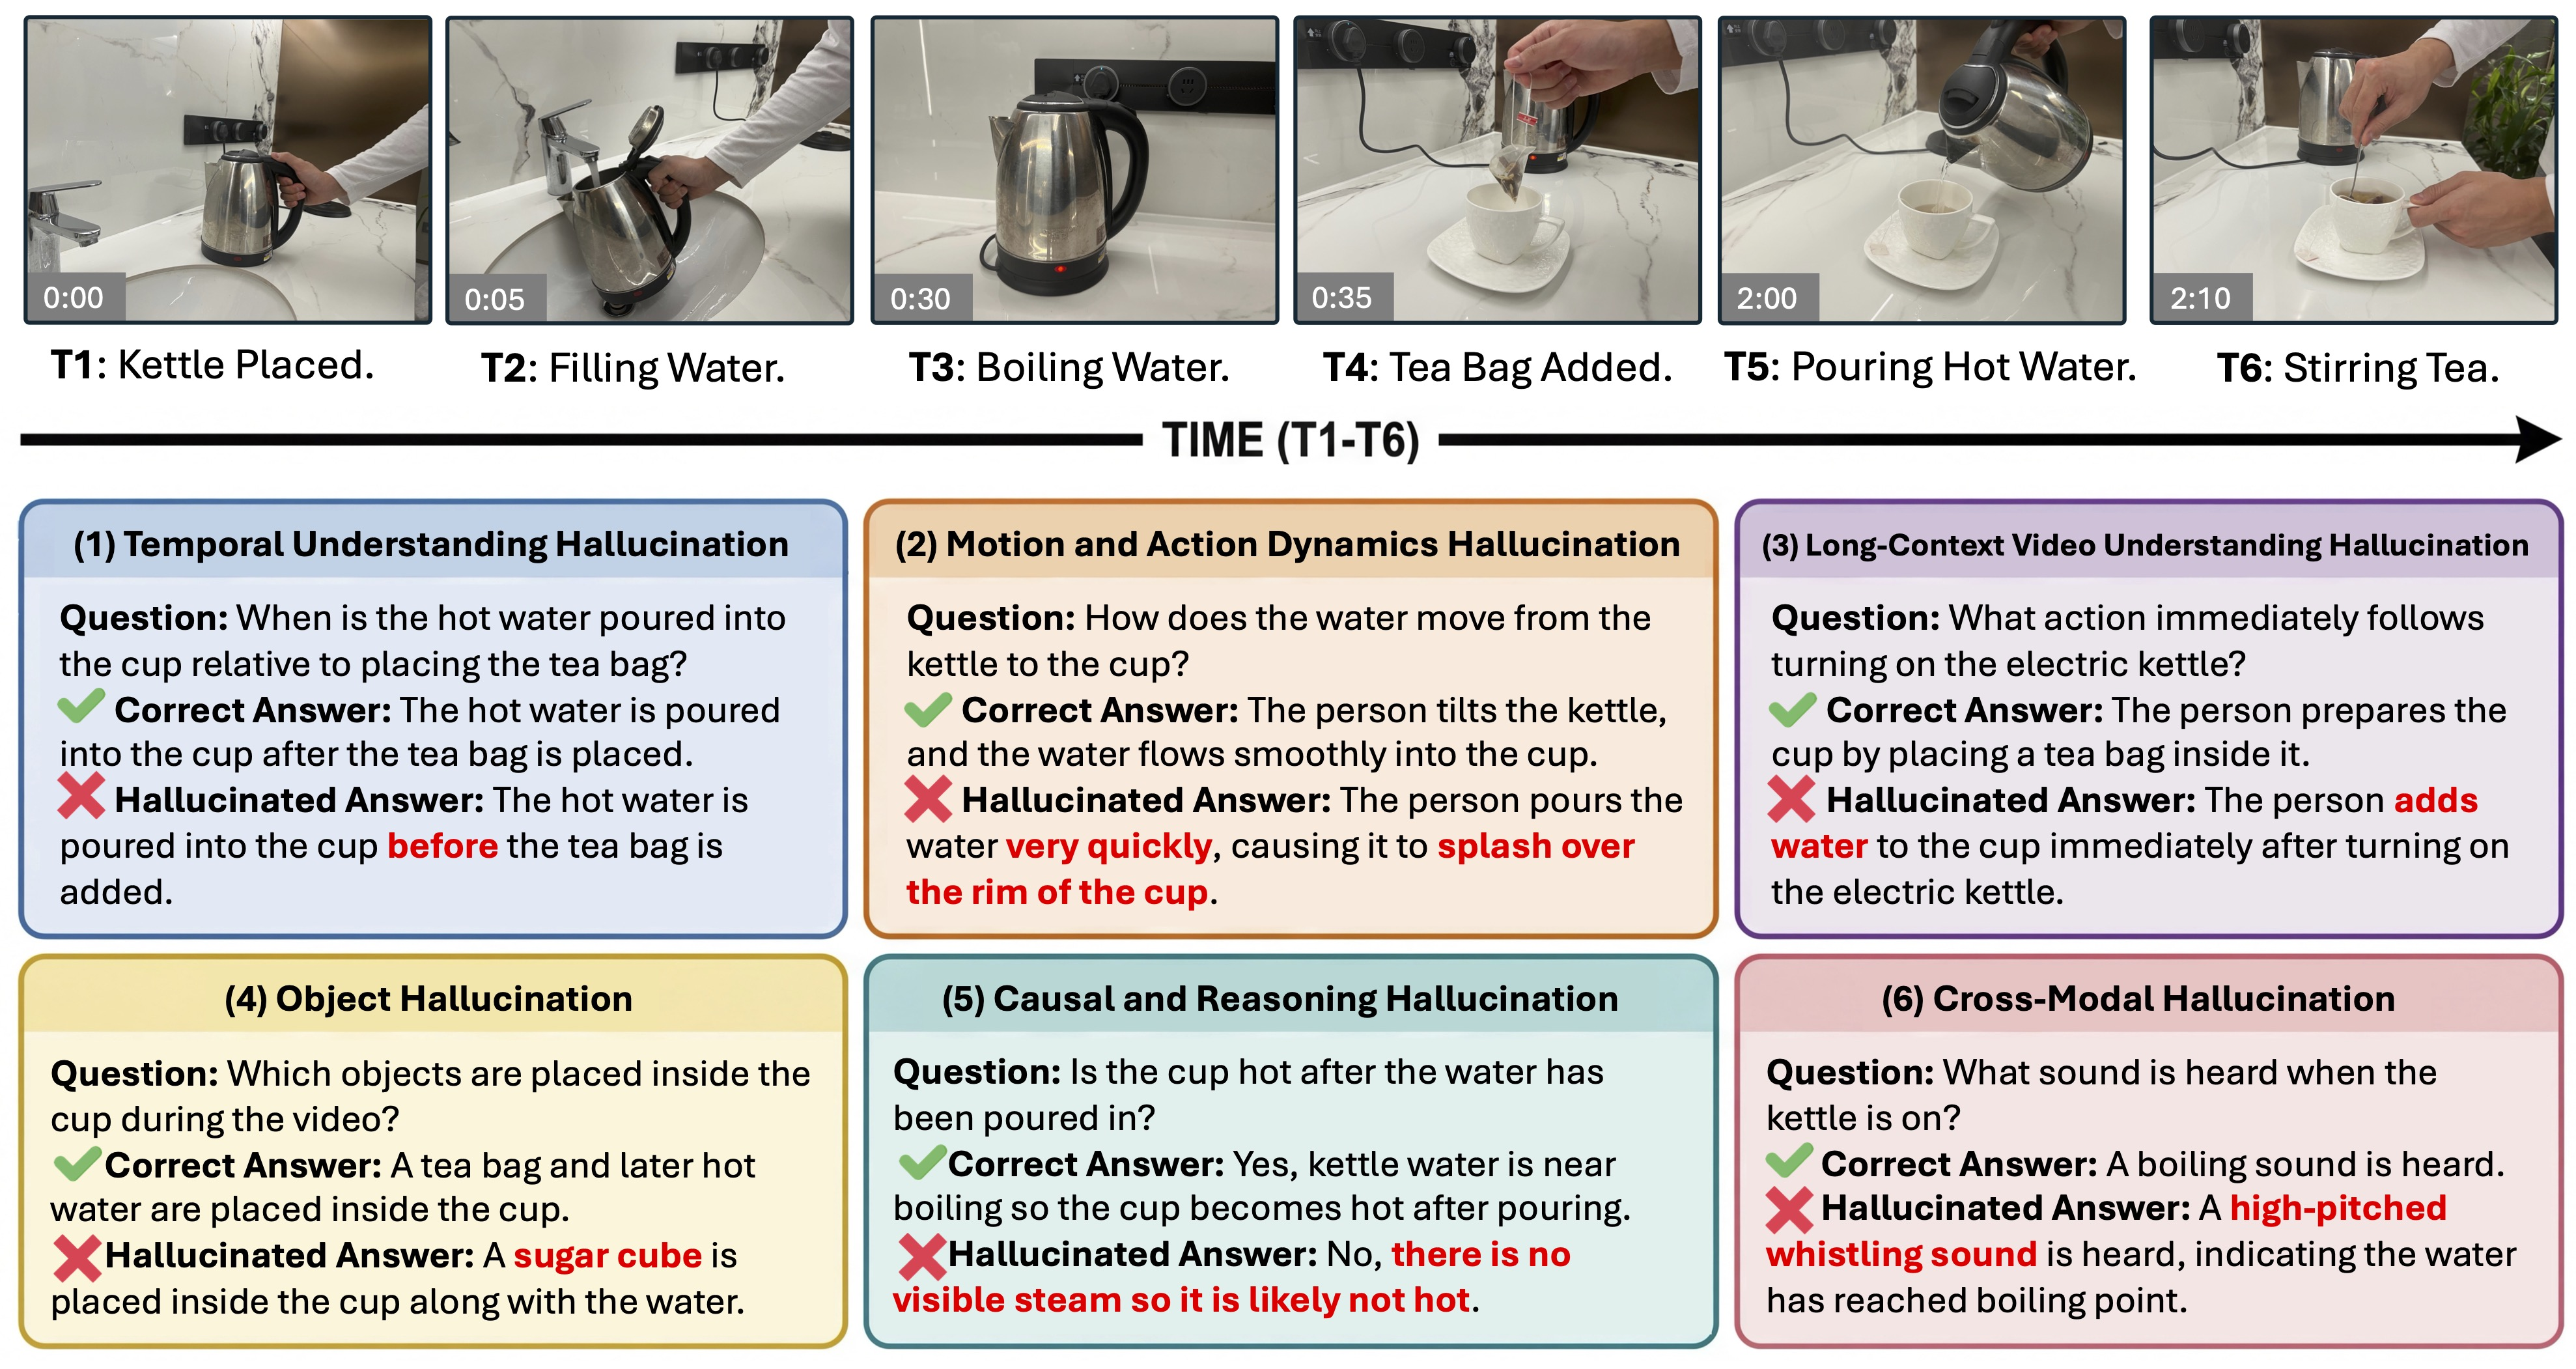
\includegraphics[width=\linewidth]{figure/hallucination_illustration_tea.pdf}
  \caption{\textbf{Simple illustration of major video-understanding hallucination types.}
  Using a tea-making example with a timeline of key moments (T1--T6), the figure contrasts correct and hallucinated answers across six categories: (1) temporal understanding hallucination, (2) motion and action dynamics hallucination, (3) long-context video understanding hallucination, (4) object hallucination, (5) causal and reasoning hallucination, and (6) cross-modal hallucination.}\label{fig:hallucination_illustration_tea}
\end{figure}

\begin{figure}[t]
  \centering
  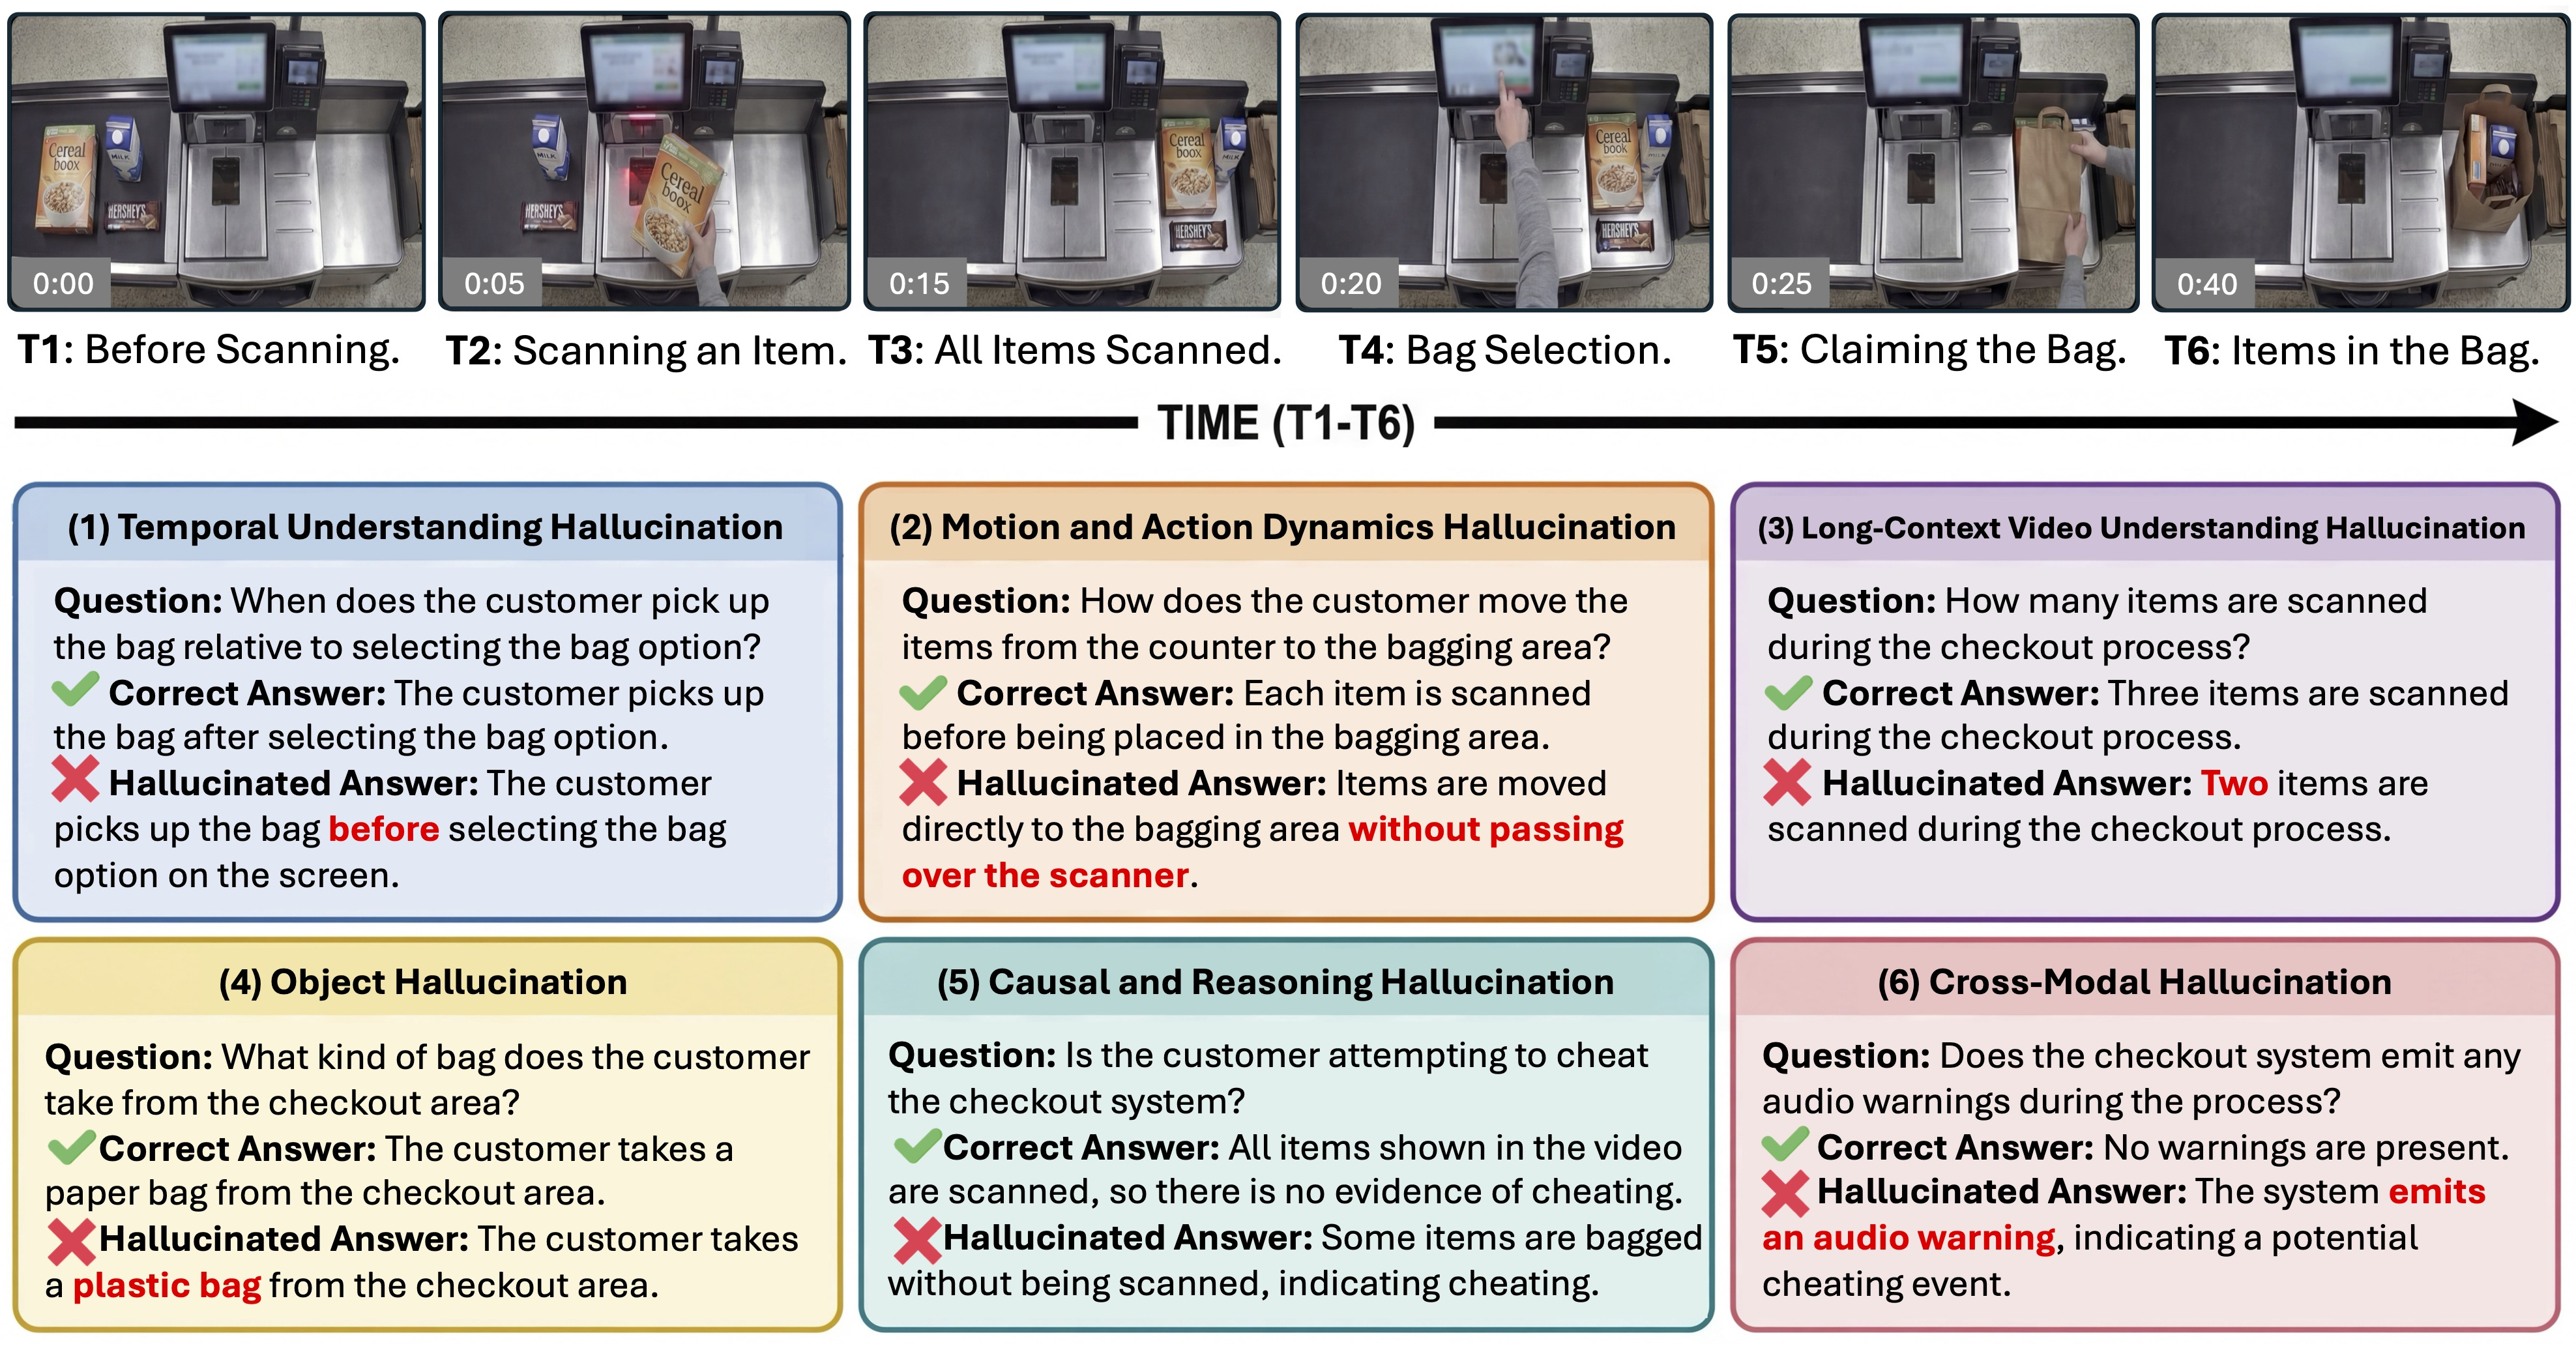
\includegraphics[width=\linewidth]{figure/hallucination_illustration_grocery.pdf}
  \caption{\textbf{Real-world example of major video-understanding hallucination types.}
  Using a grocery store self-checking example with a timeline of key moments (T1--T6), the figure contrasts correct and hallucinated answers across six categories: (1) temporal understanding hallucination, (2) motion and action dynamics hallucination, (3) long-context video understanding hallucination, (4) object hallucination, (5) causal and reasoning hallucination, and (6) cross-modal hallucination.}%
  \label{fig:hallucination_illustration_grocery}
\end{figure}

Hallucination in Vid-LLMs presents challenges far more complex than those encountered in static image understanding. % These difficulties arise from the inherent properties of video data and the architectural limitations of Vid-LLMs.

\paragraph{Temporal complexity and ambiguity.}
Videos encode information across time, where meaning depends on event order, duration, and temporal context. When models develop ambiguous temporal understanding, they infer incorrect actions or event sequences. Small temporal misalignments can propagate into large semantic hallucinations at the event level.

\paragraph{Long-context compression and memory degradation.}
Vid-LLMs may not directly process all frames in a video sequence. Instead, they rely on sampling and compression to fit input into limited tokens or memory slots to enable long-context modeling in practice. But this inevitably discards fine-grained video details. As video length increases, models forget early events, conflate attributes across distant segments, or hallucinate on details.

\paragraph{Entanglement of different errors.}
In Vid-LLMs, hallucinations may stem from incorrect or incomplete object recognition, which then propagates through downstream temporal and linguistic reasoning modules. But, even when frame-level object recognition is accurate, errors in temporal aggregation, cross-clip reasoning, or causal inference can lead to wrong conclusions, too. Therefore, perceptual, temporal, and reasoning errors are possibly entangled, which makes it challenging to determine where a hallucination originates.

% These challenges highlight that hallucination in Vid-LLMs is not merely an amplified version of image hallucination, but a distinct reliability problem. Addressing these challenges requires video-specific taxonomies and mitigation strategies, which we systematically develop in the remainder of this survey.
\section{Hallucination Taxonomy}\label{sec:hallucination-tax}

% The outline of the hallucinatino taxonomy
\input{src/figure_hallucination_taxonomy}

To systematically analyze Vid-LLMs' hallucination, we organize existing failure modes into a unified taxonomy. Figure~\ref{fig:hallucination_taxonomy} groups hallucination phenomena into six major categories. Each category captures distinct reliability failures that can arise while other aspects of video perception remain accurate.

Figures~\ref{fig:hallucination_illustration_tea} and~\ref{fig:hallucination_illustration_grocery} demonstrate different hallucination categories through concrete examples. %The first provides a simple tea-making illustration, while the second presents a real-world grocery self-checkout scenario. % For each hallucination category, we identify the most common and representative error patterns observed in practice. This explicit pairing of categories with their characteristic errors enables systematic diagnosis of model failures and provides a foundation for mapping hallucination types to targeted mitigation strategies.
\subsection{Temporal Understanding Hallucination}\label{subsec:temporal-hallucination}

Temporal understanding hallucination is the failure where a Vid-LLM produces incorrect temporal ordering or event timing. The model may correctly recognize which events are present but misrepresent their chronological order, relative timing, or durations. Prior work on temporal reasoning and moment-level understanding has shown that such temporal errors remain prevalent~\citep{ahn2025happens,huang2024vtimellm}. We identify two major manifestations of this category: \emph{sequencing errors} and \emph{temporal grounding errors}.

\paragraph{Sequencing Errors.}
Sequencing errors arise when a model messes up the chronological order of events while correctly identifying the individual events themselves~\citep{wu2025season, Plizzari2025OmniaDE, li2025vidhalluc}. A common example is ``the person sits down and then stands up'' when the video actually shows standing and then sitting. Another case is ``the player celebrates and then scores'' when the score clearly precedes the celebration.

Empirical analyses of temporal ordering have shown that models frequently struggle with maintaining consistent event order, leading to swapped or reversed narratives in generated descriptions \citep{ahn2025happens, Xue2025SeeingTA}.

\paragraph{Temporal Grounding Errors.}
Temporal grounding errors arise \emph{when} an event is claimed to happen along the timeline but assigned incorrect timestamps or boundaries. For instance, stating that ``a person starts running'' at 0:10 when it actually starts at another time, or describing that ``the accident happens in the last few seconds'' when it occurs near the middle of the video~\citep{guo2025vtg,chen2024timemarker}. Another common symptom is over-extending event duration, where a brief hand gesture is described as spanning an entire segment. These errors have been widely documented in fine-grained grounding and moment localization tasks \citep{huang2024vtimellm, wang2024grounded, wu2025number, pramanick2025enrich}.

\subsection{Motion and Action Dynamics Hallucination}
\label{subsec:motion-hallucination}

Motion and action dynamics hallucination refers to failures in capturing how movements unfold over time, which is important when to distinguishing between actions relies on subtle temporal cues or when correct understanding requires consistent modeling of physical trajectories. Such hallucinations arise when models fail to encode fine-grained inter-frame changes, causing them to hallucinate motion that never occurred or misinterpret visually similar actions. We highlight two recurring error patterns: \emph{fine-grained action errors} and \emph{physics attribute errors}.

\paragraph{Fine-Grained Action Errors.}
Even when the model understands the scene, it can fail to distinguish subtle motions~\citep{du2025motionsight, hong2025motionbench}. %Fine-grained action errors occur when the model confuses visually similar but semantically distinct actions. 
For example, describing a person as running when they are actually walking quickly, or claiming that a person is rubbing their eyes when they are merely adjusting their glasses. The literature attributes it to insufficient sensitivity to small-amplitude temporal differences across adjacent frames~\citep{shao2020finegym, liu2022fineaction}.

\paragraph{Physics Attribute Errors.}
Physics attribute errors are failures in tracking the kinematic evolution of objects~\citep{wu2025st}. Typical mistakes include stating that a ball rolls to the left when it does to the right, or stating the speed wrong. %Models may describe an object as moving rapidly when the actual motion is slow and gradual. In more complex scenarios, 
Models may also hallucinate physically implausible transitions, such as sudden direction changes without a transition.
Empirical studies such as PhyVLLM~\citep{zhan2025phyvllm} and PiTe~\citep{liu2024pite} claim that incorrect reasoning about motion direction, trajectory, and velocity remains common in Vid-LLMs.

\subsection{Long-Context Video Understanding Hallucination}\label{subsec:long-context-hallucination}

Long-context video understanding hallucination arises as its name suggests. %specifically when processing extended video inputs. 
When models integrate evidence across thousands to millions of frames, constraints from limited context windows, compressed representations, sliding windows, or limited external memory can distort what the model recalls or attends to over time. We identify three characteristic error patterns: \emph{catastrophic forgetting}, \emph{attribute merging}, and \emph{redundancy failure}.

\paragraph{Catastrophic Forgetting.}
Earlier evidence tends to gradually disappear as the model processes later frames~\citep{xiong2025streaming, wang2024videollamb}. Catastrophic forgetting occurs when a model correctly had encoded an early event or fact but later fails to recall it or produces contradictory statements~\citep{jin2025videomem, yang2025streammem, li2024videochat, yuan2025memory}. Consider an hour-long lecture video where a model correctly recognizes that the instructor taught something in the first few minutes, yet later claims it didn't happen when queried near the end.

\paragraph{Attribute Merging.}
Attribute merging refers to information \emph{conflation}, i.e., the model incorrectly blends attributes of objects, people, or scenes that appear at different times~\citep{lu2025elv}. For example, after observing a red car early and a blue car later, the model incorrectly answers with a red car in the later scene.

\paragraph{Redundancy Failure.}
Long videos often contain large volumes of repetitive or low-information frames, which can suppress attention to sparse but critical evidence~\citep{yunzhuzhang2025flexselect, hu2025m, yu2024frame}. Redundancy failure arises when models become overwhelmed by static scenes or slow-changing environments, causing salient events to get diluted, thus triggering hallucinated details~\citep{zhang2025adard, zhang2025prompt, tan2026think}. In an hour-long security camera feed with mostly event-free frames, a person may briefly walk through the hallway mid-video, yet the model fails to identify or report this event due to the dominance of redundant low-activity content. The signal-to-noise ratio becomes particularly problematic in such scenarios.

\subsection{Object Hallucination}\label{subsec:object-hallucination}

Object hallucination describes perception-level failures where a model cannot reliably extract object-centric evidence and consequently generates unsupported or inconsistent claims. Compared to static images, object understanding in videos presents greater challenges, as objects may undergo motion, occlusion, viewpoint changes, and appearance variation. Hallucination may arise in identifying \emph{what} objects exist, \emph{which} attributes they exhibit, or \emph{how} they are spatially arranged in a dynamic video setting. We summarize three representative forms of hallucination: \emph{existence errors}, \emph{attribute errors}, and \emph{spatial relation errors}.

\paragraph{Existence Errors.}
Existence errors are hallucinated objects that do not appear in the video. Temporal sparsity and occlusion often exacerbate such failures, where objects may be visible only briefly or partially, making consistent presence tracking difficult~\citep{lusha2025graph, rawal2025argus, wang2024videohallucer}. Consider a cooking video that shows only a person stirring a pot yet a model may hallucinate the presence of a knife even though no knife ever appears. This type of unsupported entity generation has been reported in~\citep{chang2025mitigating, wang2025object}.

\paragraph{Attribute Errors.}
Attribute errors refer to misidentified visual properties, such as color, shape, size, or textual content, often due to lighting variation, motion blur, and viewpoint shifts~\citep{rawal2025argus, patraucean2023perception, yang2025mesh}. The model may correctly recognize a car but incorrectly claim it is red when it is actually blue. Such errors frequently occur in long-video understanding, where incomplete or compressed representations amplify the model's confusion~\citep{wang2024videoagent, zou2024seconds}.

\paragraph{Spatial Relation Errors.}
Spatial relation errors are incorrectly described configurations or relative positions of objects. For example, it may state ``the cup is on the table'' when the video shows the cup being held in a hand. These errors may be attributed to the changing spatial groundings like object motion and camera movement~\citep{wang2024videohallucer}. Imperfect spatial grounding may cause models to generate plausible but unsupported relations~\citep{wang2025spacevllm, ouyang2025spacer, tang2025video}.

\subsection{Causal and Reasoning Hallucination}\label{subsec:reasoning-hallucination}

Causal and reasoning hallucination arises when a model produces logically unsupported conclusions on top of otherwise correct perception. Here, models hallucinate unobservable concepts such as motivations, emotions, intentions, or causal relations. Unlike object hallucination (e.g., hallucinating an object), this category reflects breakdowns in higher-level inference over events and interactions~\citep{jiang2025videop2r}. Such failures are particularly salient in video understanding because correct reasoning often requires integrating temporal cues, social context; and multi-step event structures. We identify three representative forms: \emph{false causality}, \emph{intent and emotion misattribution}, and \emph{counterfactual reasoning errors}.

\paragraph{False Causality.}
False causality is a spurious cause-to-effect link: the model correctly recognizes events but constructs an unsupported causal explanation often by relying on stereotypical correlations instead of video evidence~\citep{guda2024causal, li2022representation, chen2024mecd}. For example, seeing a video where a man suddenly starts running, the model may claim he is running because someone is chasing him. Models often conflate correlation with causation and over-rely on commonsense priors~\citep{liu2023vcd, wei2023visual}.

\paragraph{Intent and Emotion Misattribution.}
Intent and emotion misattribution is the \emph{over-interpretation of social evidence}: the model maps observable behavior into mental-state labels without sufficient visual support~\citep{li2023intentqa, ye2024dual, peng2025svbench,chen2025through, kong2025siv}. For instance, a model may claim that ``two people are arguing'' based on their gestures, when the video actually shows them laughing with gestures.

\paragraph{Counterfactual Reasoning Errors.}
Counterfactual reasoning errors emerge under \emph{hypothetical intervention} queries, where correctness requires reasoning about alternative outcomes consistent with rules and causal structure~\citep{chen2025countervqa,huang2025taming,poppi2026countervid} indicated by the video. For example, when asked ``What would happen if the player missed the shot?'', the model may hallucinate an outcome that contradicts the rules of the game played in the video.

\subsection{Cross-Modal Hallucination}\label{subsec:cross-modal-hallucination}

Cross-modal hallucination arises when models incorrectly integrate multimodal evidence (e.g., vision, audio, and text), producing outputs that violate cross-modal consistency~\citep{guo2025aligned,shen2023fine}. We categorize it into four recurring patterns: \emph{modality neglect}, \emph{audio-visual asynchrony}, \emph{audio-video grounding failure}; and \emph{false premise text--video hallucination}.

\paragraph{Modality Neglect.}
Modality neglect occurs when one modality (typically vision) dominates, causing the model to ignore another (typically audio), even when it is salient~\citep{guo2025aligned,shen2023fine, li2025watch}. For example, a video shows a person smiling and nodding while the audio contains another person saying ``I feel terrible and I need help'', but a model that discards the audio clues may output ``a person is listening and agreeing''~\citep{hanna2024multi, cheng2024videollama}.

\paragraph{Audio-Visual Asynchrony.}
Audio-visual asynchrony is a temporal alignment failure: the model uses both modalities but binds auditory evidence to the wrong visual moment~\citep{goel2024omcat, tang2025empowering}. For instance, it may describe a door slamming sound as occurring when a person merely approaches the door, rather than when the door actually closes.

\paragraph{Audio-Video Grounding Failure.}
Audio-video grounding failure concerns \emph{source attribution}: the model assigns an audio signal to an incorrect visual entity or invents a source not responsible for the sound~\citep{li2022learning,jiang2023target}. For example, in a scene with multiple people on screen and background television audio, the model may hallucinate that one of the visible individuals is speaking, rather than the off-screen TV~\citep{li2024object}.

\paragraph{False Premise Text-Video Hallucination.}
False premise text-video hallucination arises when the textual input embeds an assumption that conflicts with the video, and the model prioritizes linguistic grounding over visual grounding~\citep{gao2025exploring}. For example, when asked about the color of a cat in a video that contains no cat, the model may answer ``the cat is white,'' hallucinating to satisfy the textual premise~\citep{seth2025egoillusion}.

\section{Foundations of Hallucination Mitigation}
\label{sec:condensed_tutorial}
% Condensed Tutorial

\begin{figure}[t]
  \centering
  \includegraphics[width=0.9\linewidth]{figure/mitigation_overview.pdf}
  \caption{Illustration of representative hallucination mitigation strategies in Vid-LLMs organized by the stage of the pipeline where they intervene. Colored components highlight different methodological directions discussed in Section~\ref{sec:condensed_tutorial}, with each color corresponding to one direction, while the grey blocks depict the standard Vid-LLMs pipeline.
}
\label{fig:mitigation_overview}
\end{figure}


Before summarising specific mitigation techniques in Section~\ref{sec:mitigation} below, we review recurring methods underlying recent hallucination mitigation research. As hallucination arises from failures at different stages of the Vid-LLM pipeline, existing mitigation approaches can be understood as interventions at the corresponding stages. The following subsections review these methods, including reinforcement learning (RL) and preference optimization, supervision augmentation with synthetic data, structured representations, long-context video evidence management, and inference-time interventions, organized by where they intervene (see Figure~\ref{fig:mitigation_overview}).

\subsection{Reinforcement Learning and Preference Optimization}

RL and preference optimization align LLMs with desired behaviors by introducing training objectives beyond standard likelihood-based learning~\citep{zhang2025survey, rafailov2023direct}. The language model is treated as a policy, and an external training signal evaluates generated outputs and updates the model parameters so that preferred responses become more likely~\citep{liu2025reinforcement}.

In RL-based methods, the model generates candidate outputs and receives reward signals measuring factual correctness, reasoning quality, or human preference alignment. Policy optimization then updates the model to reinforce higher-reward responses and suppress lower-reward ones. For Vid-LLMs, effective reward design relies on verifiable supervision tied to video-specific structure, such as timestamps, segment boundaries, object trajectories, and event sequences, rather than generic answer correctness alone~\citep{Feng2025VideoR1RV, Chen2025ChronoForgeRLCF}.

Preference optimization instead trains on pairs of candidate responses where one is preferred over the other~\citep{Huang2025VistaDPOVH}. In video-language settings, many hallucinations arise from subtle temporal or spatial misalignments rather than completely wrong answers, so preference construction benefits from fine-grained temporal or motion-aware supervision rather than relying on coarse human judgments~\citep{Li2025TemporalPO, Kulkarni2025VideoPASTA7P}.

\subsection{Supervision Augmentation and Synthetic Data}

Standard video datasets emphasize coarse descriptions and contain little supervision for subtle temporal relations, object interactions, or causal reasoning. Models may therefore never encounter training examples that explicitly penalize hallucinations of these kinds.

Synthetic supervision addresses this by constructing additional training examples that highlight hallucination-prone scenarios. Synthetic pipelines perturb or recompose video-text pairs to train the model on correct evidence grounding, for instance, by shuffling or reversing event sequences~\citep{Chen2023COSACS, Vani2025HarnessingSP}, and concatenating shorter clips to simulate long videos~\citep{Ren2024VISTAEL}.

However, synthetic supervision introduces a trade-off between controllability and realism: artificially constructed examples may not reflect natural video distributions. The additional fine-grained temporal signals also increase memory and token requirements, so the effectiveness of synthetic data depends on both the quality of generated supervision and whether the model architecture can preserve these signals during long-context processing.

\subsection{Structured Representations}

Structured representations modify models to keep entities, relations, and interactions explicit during reasoning, rather than mapping visual inputs directly into dense token embeddings. Such models may benefit from intermediate, interpretable structures like relational graphs, modular feature groups, and entity-based representations~\citep{Mao2022DynamicMR}.

In video understanding, hallucinations can be attributed to planning errors, not only perception errors, for example, answering before it has localized the relevant moments or decomposed the reasoning path. Structured representations help because they force intermediate grounding decisions before the final answer. An effective design to address the issue links observations across multiple frames into temporally coherent units through temporal linking, trajectory aggregation, or timestamp-aware embeddings; they encode both appearance features and temporal indices~\citep{Guo2025VTGLLMIT, Wang2024GroundedVideoLLMSF}.

Another approach organizes video information into scene graphs or dynamic interaction graphs, representing entities as nodes and their spatial or temporal interactions as edges~\citep{Du2025SceneawareGM}. Reasoning over explicit relationships helps prevent the model from introducing unsupported objects, relations, or interactions~\citep{Huang2025BuildingAM, Chu2025GraphVideoAgentEL}.

In practice, structured representations alone are insufficient. Their effectiveness depends on how the model uses them, which require trainings or agent pipelines that focus attention on query-relevant relations and evidence~\citep{Malik2025RAVURA}.

\subsection{Long-Context Information Management}

Long videos introduce a fundamental challenge: a single video may contain thousands of frames, while the model can process only a limited number of visual tokens~\citep{Xu2025EVRAGEL}. Models must therefore selectively retain, compress, and retrieve information from earlier parts of the video.

Memory-based approaches augment the model with external or persistent memory that stores compact representations of previously processed segments, such as learned embeddings, key-value representations, and segment-level summaries. At query time, relevant memory entries are retrieved through similarity matching~\citep{Song2023MovieChatFD, Jin2025VideoMemEU}.

Token compression methods reduce visual tokens by merging redundant tokens using clustering, similarity-based merging, or learned compressors, fitting longer videos within fixed context budgets~\citep{Weng2024LongVLMEL, Guo2025FiLAVideoSC}. Empirically, effective compression preserves the spatial and temporal structure of events rather than minimizing token counts uniformly, because collapsing distinct moments into indistinguishable tokens can lead to hallucinated actions or causal relations~\citep{Sun2025LLaVAScissorTC}.

Hallucination in long videos can also be a retrieval failure disguised as a reasoning failure~\citep{yu2026longvidsearch}. Frame selection methods estimate frame relevance using motion cues, saliency scores, or query-conditioned scoring and select informative subsets for reasoning~\citep{Tang2025AdaptiveKS, Guo2025LogicinFramesDK}. Retrieval-based pipelines index video segments externally and retrieve the most relevant clips for the query~\citep{Ataallah2024GoldfishVU, Yuan2025MemoryenhancedRA}.

\subsection{Inference-Time Intervention}

Inference-time intervention methods work during generation instead of training, which has been popular in recent years in all LLM modalities. Chain-of-thought (CoT) prompting, for example, inserts reasoning demonstrations or instructions such as ``think step by step'' to structure how the model produces tokens~\citep{wei2022chain, zhang2022automatic}.

For Vid-LLMs, the prompt encourages intermediate reasoning steps that reference specific video observations, e.g., events, object interactions, and temporal relations, before integrating them into a final conclusion~\citep{Zhang2025ViTCoTVI,jin2025cot}.

Beyond linear reasoning traces, agentic reasoning procedures organize inference as an iterative loop of planning, tool calling, and result updating~\citep{luo2025large, huang2024understanding, ishibashi2024self}. In video understanding, as we mentioned before, hallucination often arises from failures in summarization and planning rather than perception. Agentic frameworks address this by first planning which parts of the video to inspect, then performing targeted operations such as selecting relevant frames or retrieving supporting segments~\citep{Zhang2025ThinkingWV, Chen2025LVAgentLV}. The final answer is produced only after sufficient visual evidence has been collected.

\section{Mitigation Techniques}\label{sec:mitigation}

\input{src/figure_mitigation_taxonomy}

We now review concrete mitigation techniques organized according to the hallucination categories from Section~\ref{sec:hallucination-tax}, examining how different methods improve model faithfulness and reliability (see Figure~\ref{fig:mitigation_technique}).

\subsection{Temporal Understanding Hallucination Mitigation}\label{subsec:temporal-hallucination-mitigation}

\begin{figure}[t]
  \centering
  \includegraphics[width=0.95\linewidth]{figure/temporal_hallucination_mitigation_illustration.pdf}
  \caption{Illustration of representative strategies for mitigating temporal understanding hallucinations in Vid-LLMs. (a) Preference optimization and reinforcement learning methods enforce temporally grounded reasoning by rewarding correct frame ordering and penalizing temporally inconsistent predictions. (b) Temporal structure modeling introduces dedicated temporal encoders or time-aware representations that explicitly capture event ordering and timestamp information for downstream reasoning. (c) Synthetic temporal augmentation improves robustness by exposing the model to temporally perturbed training samples, such as reversed or shuffled event sequences.}
  \vspace{-3mm}
\label{fig:mitigation_temporal_hallucination}
\end{figure}

Temporal understanding hallucination is a major failure mode of Vid-LLMs, motivating the inventions of techniques that target temporal ordering, localization, and duration grounding. Existing approaches fall into three technical paradigms: (i)~\emph{preference optimization and reinforcement learning} with temporally grounded reward signals; (ii)~\emph{specialized architectures and inference-time interventions} that encode or diagnose temporal structure; (iii)~\emph{synthetic data generation and spatiotemporal augmentation} to expose models to temporally perturbed supervision (see Figure~\ref{fig:mitigation_temporal_hallucination}).

\paragraph{Preference Optimization and Reinforcement Learning}

Early supervised fine-tuning approaches such as TimeChat~\citep{Ren2023TimeChatAT} and TRACE~\citep{Guo2024TRACETG} penalize false negatives under autoregressive losses, causing overfitting and poor generalization. RL-based alternatives are motivated by the insight that temporal localization quality is better captured by task-specific reward signals than by token-level cross-entropy.

Time-R1~\citep{Wang2025TimeR1PL} post-trains Vid-LLMs using RL with verifiable rewards (RLVR), combining a timestamp-aware Intersection-over-Union (tIoU) signal with a reasoning-template reward optimized via Group Relative Policy Optimization (GRPO). On Charades-STA~\citep{gao2017tall}, Time-R1 achieves R1@0.7 of 35.3, roughly doubling TRACE and nearly tripling TimeChat. It reduces hallucination rates by 10--15\% from baselines. Temporal grounding improves when the model is rewarded for evidence-consistent temporal decisions rather than matching surface-form annotations. TimeZero~\citep{Wang2025TimeZeroTV} demonstrates that structured RL-guided reasoning can yield competitive temporal localization from as few as 2,500 training samples. However, both methods incur higher training and inference costs and struggle with ultra-long video contexts.

D$^2$VLM~\citep{Zeng2025FactorizedLF} addresses the entanglement between temporal grounding and text generation by decoupling these objectives through explicit evidence tokens that capture event-level visual semantics, forcing the model to obtain temporal evidence before generating an answer. This improves grounding accuracy over TimeChat-7B~\citep{ren2024timechat} with only 1.4\% computational overhead per token, though performance on episodic memory and fine-grained event boundary detection remains limited.

Subsequent work refines the RL approach along several axes. VideoChat-R1~\citep{Li2025VideoChatR1ES} extends to multi-task reinforcement fine-tuning, jointly optimizing temporal grounding, object tracking, and question-answering, yielding gains over Video-R1~\citep{Feng2025VideoR1RV}. MOSSChat-V~\citep{Tao2025MOSSChatVRL} addresses ``temporal hacking'', where models bypass temporal reasoning to guess outcomes directly, through a process-reasoning reward based on subsequence Dynamic Time Warping (DTW) that supervises intermediate temporal logic. \citet{Li2025ReinforcementLT} combine discrete semantic rewards with continuous tIoU signals alongside variance-aware data selection, surpassing Video-R1 on temporal grounding with substantially less training data.

Additional efforts explore hybrid off-policy sampling and soft advantage estimation~\citep{Li2025TempSampR1ET}, multi-task RL with task-specific localization rewards~\citep{Wu2025TempR1IT}, and metric-based direct preference optimization through chain-of-tasks decomposition~\citep{Lee2025VidChainCW}. These studies confirm a shift from static supervised objectives toward adaptive, reward-driven post-training. The main strength is its flexibility: post-training alignment can layer on top of existing Vid-LLMs without architectural redesign. On the other hand, reliable rewards are very tricky to design, long-horizon reasoning increases training instability, and scalability to ultra-long contexts remains very challenging.

\paragraph{Specialized Architecture and Inference-Time Intervention}

Architectural approaches modify what the model \emph{represents} by embedding temporal structure directly into its token vocabulary, attention mechanisms, or decoding pipeline. Their thought was, if time is only weakly encoded in the input, no amount of post hoc alignment can fully recover precise chronology.

Early work VTimeLLM~\citep{Huang2023VTimeLLMEL} introduced a three-stage curriculum that progressively sharpens temporal perception through dedicated boundary detection tasks, improving temporal grounding over Video-LLaMA~\citep{Zhang2023VideoLLaMAAI}. Models that recognize content well may still fail to segment event boundaries, indicating that temporal hallucination is partly representational. However, VTimeLLM represents timestamps as plain text and relies on detected shot boundaries, limiting intra-shot precision.

LITA~\citep{Huang2024LITALI} combines relative time tokens with a SlowFast architecture, compressing the token count from 25,600 to 356 while nearly doubling mIoU on ActivityNet-RTL~\citep{huang2024lita}. Chrono~\citep{Rodriguez2024ChronoAS} shows that a simpler, model-agnostic approach---interleaving frame embeddings with absolute integer timestamps---can outperform complex specialized modules with only 19M trainable parameters via LoRA. These results suggest that some temporal hallucinations arise not from weak visual features but from the model's inability to interpret temporal metadata. Grounded-VideoLLM~\citep{Wang2024GroundedVideoLLMSF} extends this with a dual-stream architecture that encodes spatial and temporal components through discrete temporal tokens sharing an embedding space with the language model.

VTG-LLM~\citep{Guo2024VTGLLMIT, Guo2025VTGLLMIT} tackles concept shifts from identical output targets for varying inputs by integrating sequence-time embeddings, absolute-time tokens, and slot-based compression enabling denser frame sampling without expanding the context window. GeLM~\citep{Chen2024GroundedMV} augments the vocabulary with dynamic grounding token pairs fused with visual features through a dual-branch saliency-similarity module, more than doubling IoU@0.3 on MULTIHOP-EGOQA~\citep{chen2025grounded} relative to TimeChat~\citep{ren2024timechat}, which is important for settings where the answer depends on several disjoint moments.

Two recent directions go beyond discrete tokens. VTune~\citep{Jung2024OnTC} reformulates temporal grounding as a verification process requiring models to confirm or correct query-moment alignments at inference time, substantially improving TimeChat's consistency on Charades-CON~\citep{jung2025consistency}---revealing that specialized timestamp encoding alone does not guarantee robust temporal comprehension. DisTime~\citep{Zeng2025DisTimeDT} models time as continuous probability distributions rather than discrete tokens: its distribution-based decoder handles boundary ambiguity while adding less than 1\% additional parameters, surpassing discrete-quantization methods on Charades-STA~\citep{gao2017tall}. Continuous decoding is better suited to uncertain or gradually evolving events, though it remains constrained by frame-level evidence accuracy.

Complementary refinements include iterative timestamp refinement with auxiliary regression losses~\citep{Wang2024TimeRefineTG}. The field traces a trajectory from text-based timestamps through discrete tokens and dual-stream architectures to continuous distributional modeling. Architectural methods offer stronger temporal inductive bias than post-training alignment, but require more invasive modifications or denser visual processing. A promising direction is unifying these encoding paradigms for fine-grained boundary localization, multi-hop reasoning, and verification-based consistency without task-specific modifications.

\paragraph{Synthetic Data and Spatiotemporal Augmentation}

Data-centric approaches tackle temporal hallucinations at their source: the training distribution. These methods create supervision that foregrounds order, progression, and temporal coherence through synthetic or augmented videos with controlled temporal variations.

Sparrow~\citep{Yin2024SparrowDV} augments real videos with synthetic text-to-image sequences---rendering instructions as image sequences mimicking video frames---reducing required training samples by 85\% while improving temporal reasoning on Video-MME over Video-ChatGPT~\citep{Maaz2023VideoChatGPTTD}. VISTA~\citep{Ren2024VISTAEL} and COSA~\citep{Chen2023COSACS} address models trained on short clips that fail on long videos by constructing pseudo long-form sequences from short samples, strengthening event-level alignment without large native long-video corpora.

TimeWarp~\citep{Vani2025HarnessingSP} generates preference pairs by shuffling and reversing event sequences within video narratives, extending the STIC~\citep{deng2024enhancing} self-training framework to video. This reduces hallucination rates by 7.5\% on temporal benchmarks at a cost of approximately 60 A100 GPU hours per model. It is particularly effective against shortcut learning, where a model answers correctly from scene cues while ignoring chronology. Complementary works inject temporally sensitive tasks to reduce reliance on static visual bias~\citep{Wang2025TIMETM, Zhou2025StreferEV}. Perturbation-based augmentation exposes whether the model truly understands sequence order, though aggressive perturbations can drift from realistic video dynamics.

A third branch shifts from recognition to prediction. Next-Event Prediction (NEP)~\citep{Wang2025FosteringVR} trains models to generate textual summaries of future video segments conditioned on past frames, forcing internalization of event dynamics and causal progression. DIBS~\citep{Wu2024DIBSED} pursues a similar goal through diverse LLM-generated event-centric pseudo captions with online boundary refinement.

T3~\citep{Li2024TemporalRT} finds that the temporal reasoning bottleneck often resides in the language model rather than the visual encoder: by synthesizing diverse temporal tasks in pure text from image-text datasets, T3 surpasses ShareGPT4Video~\citep{Chen2024ShareGPT4VideoIV} on TempCompass~\citep{liu2024tempcompass} without any video data.

Data-centric approaches are more scalable than RL and less invasive than architectural redesign, but if synthetic supervision contains temporal bias or implausible event chains, it can regularize the model in the wrong direction. Careful control over temporal structure---through perturbation, composition, or modality transfer---proves more important than sheer data volume.

% \textbf{Summary.} The three paradigms offer complementary trade-offs. RL and preference optimization directly penalize temporal errors but require careful reward design and incur higher training costs. Architectural interventions embed temporal structure into representations, from discrete tokens to continuous distributions, but risk task-specific fragmentation. Synthetic data approaches are the most scalable, but their effectiveness depends on the quality of generated temporal variations. These strategies are not mutually exclusive: explicit temporal representations support better rewards, while synthetic counterfactuals expose failures that alignment alone misses.

\subsection{Motion and Action Dynamics Hallucination Mitigation}
\label{subsec:motion-hallucination-mitigation}

\begin{figure}[t]
  \centering
  \includegraphics[width=1.0\linewidth]{figure/motion_hallucination_mitigation_illustration.pdf}
  \caption{Illustration of representative methods for mitigating motion and action dynamics hallucinations in Vid-LLMs. Each panel depicts a representative strategy corresponding to one category discussed in this subsection, including object-centric tracking, specialized motion architectures, graph-based reasoning, dynamic token manipulation and visual prompting, reinforcement learning and preference optimization, and physics-informed modeling.}
  \vspace{-3mm}
\label{fig:mitigation_motion_hallucination}
\end{figure}

Motion and action dynamics hallucination emerges when Vid-LLMs fail to capture fine-grained temporal evolution, object trajectories, and physically grounded motion patterns. We group existing mitigation techniques into six categories (see Figure~\ref{fig:mitigation_motion_hallucination}): (i) \emph{object-centric tracking}; (ii) \emph{specialized motion architectures}; (iii) \emph{graph-based reasoning}; (iv) \emph{dynamic token manipulation and visual prompting}; (v) \emph{reinforcement learning and preference optimization}; and (vi) \emph{physics-informed modeling and 4D reconstruction}.

\paragraph{Object-Centric Tracking}

Object-centric tracking replaces coarse frame-level features with explicit per-entity trajectory representations, since action errors often stem from the model not knowing who moved, where, and in what order. PiTe~\citep{Liu2024PiTePA} tracks three key points per object across frames and projects these trajectories into the language embedding space via a dedicated trajectory projector. Supported by an automatic annotation pipeline yielding the PiTe-143k dataset and $k$-means++ clustering to manage computational overhead, PiTe demonstrates superior zero-shot performance on video question answering, temporal grounding, and dense captioning compared to static-alignment baselines such as Video-LLaMA~\citep{Zhang2023VideoLLaMAAI}. However, its reliance on sparse keypoint tracking limits performance with small or heavily occluded objects.

VideoOrion~\citep{Feng2024VideoOrionTO} extends to full object-centric tokenization through a two-branch design: a video-centric branch captures global context while an object-centric branch leverages a detect-segment-track pipeline (GroundingDINO, SAM, XMem) to extract disentangled object tokens. This substantially improves performance across MVBench~\citep{li2024mvbench}, EgoSchema~\citep{mangalam2023egoschema}, Perception-Test~\citep{patraucean2023perception}, VideoMME~\citep{fu2025video}, and ActivityNet-QA~\citep{yu2019activitynet} over spatial-temporal pooling baselines, at a roughly 38\% increase in computation time.

iMOVE~\citep{Li2025iMOVEIV} introduces the first motion-aware instruction-tuning dataset (iMOVE-IT) with fine-grained instance spatiotemporal annotations, paired with Event-aware Spatiotemporal Efficient Modeling and Relative Spatiotemporal Position Tokens. This reduces visual tokens by over 34\% via adaptive pooling while preserving motion fidelity, and unifies spatial grounding, temporal grounding, and dynamic captioning through mutual-supervision tasks. However, fixed event segmentation granularity limits applicability to ultra-long videos. The key lesson: object grounding is most effective when architecture and training data are jointly designed around motion.

Tracklet-phrase contrastive alignment~\citep{Chang2025MitigatingOA} improves object and action F1 on MiraData-9k~\citep{ju2024miradata} over Vista-LLaMA~\citep{Ma2023VistallamaRH}. Complementary works include trajectory-guided attention for detecting physical implausibility~\citep{Motamed2025TRAVLAR} and slot-based tokenization of object dynamics~\citep{Xu2024SlotVLMSS}. MotionBench~\citep{Hong2025MotionBenchBA} exposes remaining limitations on fine-grained motion tasks. These approaches force temporal reasoning to be indexed by entities instead of latent global tokens; their main limitation is scalability in crowded scenes, under heavy occlusion, or with amorphous motion regions.

\paragraph{Specialized Motion Architectures}

Whereas object-centric tracking augments the input representation, specialized motion architectures modify the model's internal processing pathways to better capture high-frequency inter-frame dynamics. \citet{Rasekh2025EnhancingTU} observed that joint spatiotemporal attention, as in InternVideo2-Chat~\citep{Wang2024InternVideo2SF}, is insufficient for distinguishing temporally mirrored actions. Their STAVEQ2 integrates stacked temporal attention (STA) modules within the vision encoder, processing patch embeddings across frames before tokens reach the language model, achieving an 11-point accuracy gain on SSv2-T10 with up to four times fewer attention heads. Early temporal processing is critical when mirrored or near-identical actions must be distinguished, though performance degrades on extremely long videos.

MASH-VLM~\citep{Bae2025MASHVLMMA} instead targets entangled causal attention within the language model: DST-attention restricts direct interactions between spatial and temporal tokens, while Harmonic-RoPE harmonizes positional IDs across multimodal tokens. This reduces hallucination rates by 12--17\% on UNSCENE~\citep{Bae2025MASHVLMMA} but remains constrained by fixed token budgets beyond 100 frames.

Complementary refinements include: a GOP encoder jointly fusing RGB and motion features within group-of-pictures units~\citep{Zhao2025EfficientMV}, surpassing Video-LaVIT's~\citep{Jin2024VideoLaVITUV} concatenation-based fusion; a diffusion-powered continuous video tokenizer preserving spatial-temporal dynamics~\citep{Ge2024DivotDP}; an appearance-free optical flow stream with action-centric contrastive learning~\citep{Chen2023ATMAT}, improving NExT-QA~\citep{xiao2021next} accuracy from 55\% to 58\%; and disentangled frame-level and motion-level features through noun-verb grounding~\citep{Liu2024VideoQA}.

At the systems level, \citet{Li2025ImprovingLV} enable 16 FPS processing via a high-frame-rate aligner with block matrix decomposition, while \citet{Hu2025SF2TSF} improve fine-grained sensitivity through self-supervised fragment-level tasks. The central trade-off is computational: motion-specialized encoders improve fidelity but increase memory use, reduce compatibility with generic backbones, or degrade on very long videos.

\paragraph{Graph-Based Reasoning}

Graph-based methods construct explicit structured representations, such as scene graphs where nodes encode objects and edges capture spatial or temporal relationships, to enable reasoning about fine-grained interactions rather than implicit holistic feature matching. Finsta~\citep{Fei2024EnhancingVR} represents both texts and videos as fine-grained scene graph structures unified into a holistic graph, with a spatial-temporal Gaussian differential Graph Transformer that differentiates between moving and stationary objects~\citep{Sun2022LongFormVP}. This improves long-form video QA accuracy by 7--9\% over the base Vid-LLM, but its performance degrades with noisy annotations and videos containing more than eight sequential actions.

GHR-VQA~\citep{Brilli2025GHRVQAGH} constructs human-rooted video-level graphs linking frame-level scene graphs via human nodes to a global root, with a hierarchical Conditional Relational Network and HetEdgeGAT encoder for cross-frame message passing. This achieves substantial gains on AGQA~\citep{grunde2021agqa} over prior graph-based approaches~\citep{Khan2023LearningSH}, since many motion questions are implicitly actor-centric. However, the single-root constraint limits scalability to multi-actor scenes.

Video-STR~\citep{Wang2025VideoSTRRM} bridges graph-based reasoning with RL by constructing inter-object relation graphs and training via GRPO with task-specific rewards. Its rotation-invariant graph representation addresses the lack of explicit spatial rewards in Video-R1~\citep{Feng2025VideoR1RV}, though graph construction introduces computational overhead.

Further extensions in this category include: a dynamic graph transformer modeling object-level temporal dynamics~\citep{Xiao2022VideoGT} beyond the static graphs of HQGA~\citep{Peng2022MultilevelHN}; temporally coherent event graphs preserving trajectory and velocity attributes~\citep{Masala2025FromVT}; multi-scale temporal modeling with visual-action semantic-aware modules~\citep{Liu2025CapturingRB}; relation-aware graph attention mechanisms~\citep{Wang2023ReGRRG}; and motion-focused video-language learning with verb-variation strategies~\citep{Doughty2024LocoMotionLM}. Graph-based approaches excel at compositional questions involving contact, order, or multi-object dependencies, but noisy detections and annotation errors can themselves become a source of hallucination. Hence, graph reasoning is most useful when paired with stronger perceptual front ends.

\paragraph{Dynamic Token Manipulation and Visual Prompting}

A complementary line of work manipulates visual token representations or augments input with explicit visual prompts that direct attention toward active motion regions. DynImg~\citep{Bao2025DynImgKF} composes key frames into a single dynamic image while using non-key frames as pixel-level temporal prompts highlighting rapidly changing regions, with a 4D rotary positional embedding preserving spatiotemporal order. Unlike Video-ChatGPT~\citep{Maaz2023VideoChatGPTTD} and Video-LLaMA~\citep{Zhang2023VideoLLaMAAI}, DynImg enables fine-grained pixel-level interactions before feature extraction, achieving substantial gains on MVBench motion subtasks. It performance starts to degrade when more than four non-key frames are used.

MotionSight~\citep{Du2025MotionSightBF} decouples object motion from camera motion at zero-shot inference time, since models often hallucinate object movement when the real cause is so-called ego-motion, i.e., the motion of a camera relative to its environment. This yields a 14.3\% gain on camera motion tasks in MotionBench~\citep{Hong2025MotionBenchBA} with modest additional inference latency. ST-LLM~\citep{Liu2024STLLMLL} shows that LLMs can directly model spatial-temporal token sequences without additional temporal modules, using dynamic masking for masked video modeling that improves MVBench~\citep{li2024mvbench} accuracy over module-heavy approaches~\citep{Luo2023ValleyVA}. Domain-specific heuristic prompts~\citep{Yu2024PromptingVF} offer lightweight alternatives. These methods are training-free with minimally invasive front-end corrections. On the other hand, when motion salience is ambiguous, manually designed prompting can suppress useful context as easily as it highlights relevant change.

\paragraph{Reinforcement Learning and Preference Optimization}

RL and preference optimization penalize incorrect action dynamics through motion-sensitive reward signals. Standard final-answer rewards are too coarse to penalize subtle mistakes in trajectory or event ordering. Invert4TVG~\citep{Chen2025Invert4TVGAT} augments RL training with verb completion, action recognition, and video description, which are derived from grounding annotations without external supervision. It reinforces action-semantic consistency while reducing GPU memory by 15\%.

VideoCap-R1~\citep{Meng2025VideoCapR1EM} extends RL to open-ended captioning through GRPO with a structured thinking paradigm, using dual reward mechanisms that includes an LLM-free think scorer and an LLM-assisted caption scorer, to yield strong F1 improvements on CAREBENCH~\citep{xu2024carebench} with only 1.5k training samples. Video-CoM~\citep{Rasheed2025VideoCoMIV} introduces a Chain of Manipulations enabling iterative visual interactions through temporal segment finding, keyframe isolation, and spatial zooming, supervised by step-level rewards for temporal IoU, frame recall, and spatial IoU. It is effective because motion understanding is often a sequential search problem.

VideoPerceiver~\citep{Zhao2025VideoPerceiverEF} enhances temporal sensitivity through key-information-absent video construction and contrastive learning, then applies a comparative GRPO reward enforcing superior response quality from complete videos over temporally degraded inputs. This yields a 22.9\% improvement on VRU-Accident~\citep{kim2025vru} with considerable computational overhead. VDCAgent~\citep{Wang2025VDCAgentWV} eliminates dependence on expensive external models via agentic self-reflection and curriculum DPO, while OwlCap~\citep{Zhong2025OwlCapHM} proposes a Caption Set Equivalence Reward jointly optimizing correctness and completeness beyond motion-only~\citep{Wang2024TarsierRF} or event-coverage-only rewards.

These works together represent a shift from task-specific binary rewards to rewards that capture subtle physical plausibility constraints (trajectory consistency, velocity coherence, biomechanical feasibility, etc.) together with external annotators at affordable costs.

\paragraph{Physics-Informed Modeling}

Physics-informed modeling directly embeds geometric and physical priors into the reasoning pipeline, constraining the hypothesis space so that implausible motion interpretations are rejected. \citet{Zhou2025LearningTR} address Vid-LLMs' inability to perform dynamic spatial reasoning by introducing the DSR Suite framework with an automated training data pipeline and a Geometry Selection Module employing two stacked Q-Formers. The module condenses question semantics and selectively extracts task-relevant geometric knowledge from 4D reconstruction priors, introducing only 32 geometry tokens to balance information density and computational cost.
MASS~\citep{Wu2025MASSMS} extends this with depth-based 3D encoding, visual grounding, and an explicit motion tracker. PhyVLLM~\citep{Zhan2025PhyVLLMPV} further extends them with continuous-time modeling through motion-appearance disentanglement, Neural ODE-based dynamics, and self-supervised physical consistency losses.

The difficulty lies upstream: physics-informed methods depend on the quality of depth estimation, reconstruction, or motion decomposition. When these priors are noisy, the model will inherit more errors than flexible learned features would. The challenge is making integration uncertainty-aware and robust to real-world sensing noise.

\textbf{Summary.} These reviewed mitigations differ in where they intervene: object-centric tracking and specialized architectures strengthen perception; graph-based reasoning and physics-informed modeling impose structure on interpretation; dynamic token manipulation offers cheaper inference-time correction; and RL reshapes training objectives toward motion-sensitive fidelity. Tracking and graph pipelines improve grounding but add preprocessing cost; specialized architectures improve accuracy but reduce efficiency; prompting is lightweight but heuristic; and RL is certainly powerful but expensive. A promising direction is, perhaps, a hybrid design: tracked or prompted motion cues feeding structured reasoning, with lightweight preference signals and uncertainty-aware physical priors.


\subsection{Long-Context Video Understanding Hallucination Mitigation}
\label{subsec:long-context-hallucination-mitigation}

\begin{figure}[t]
  \centering
  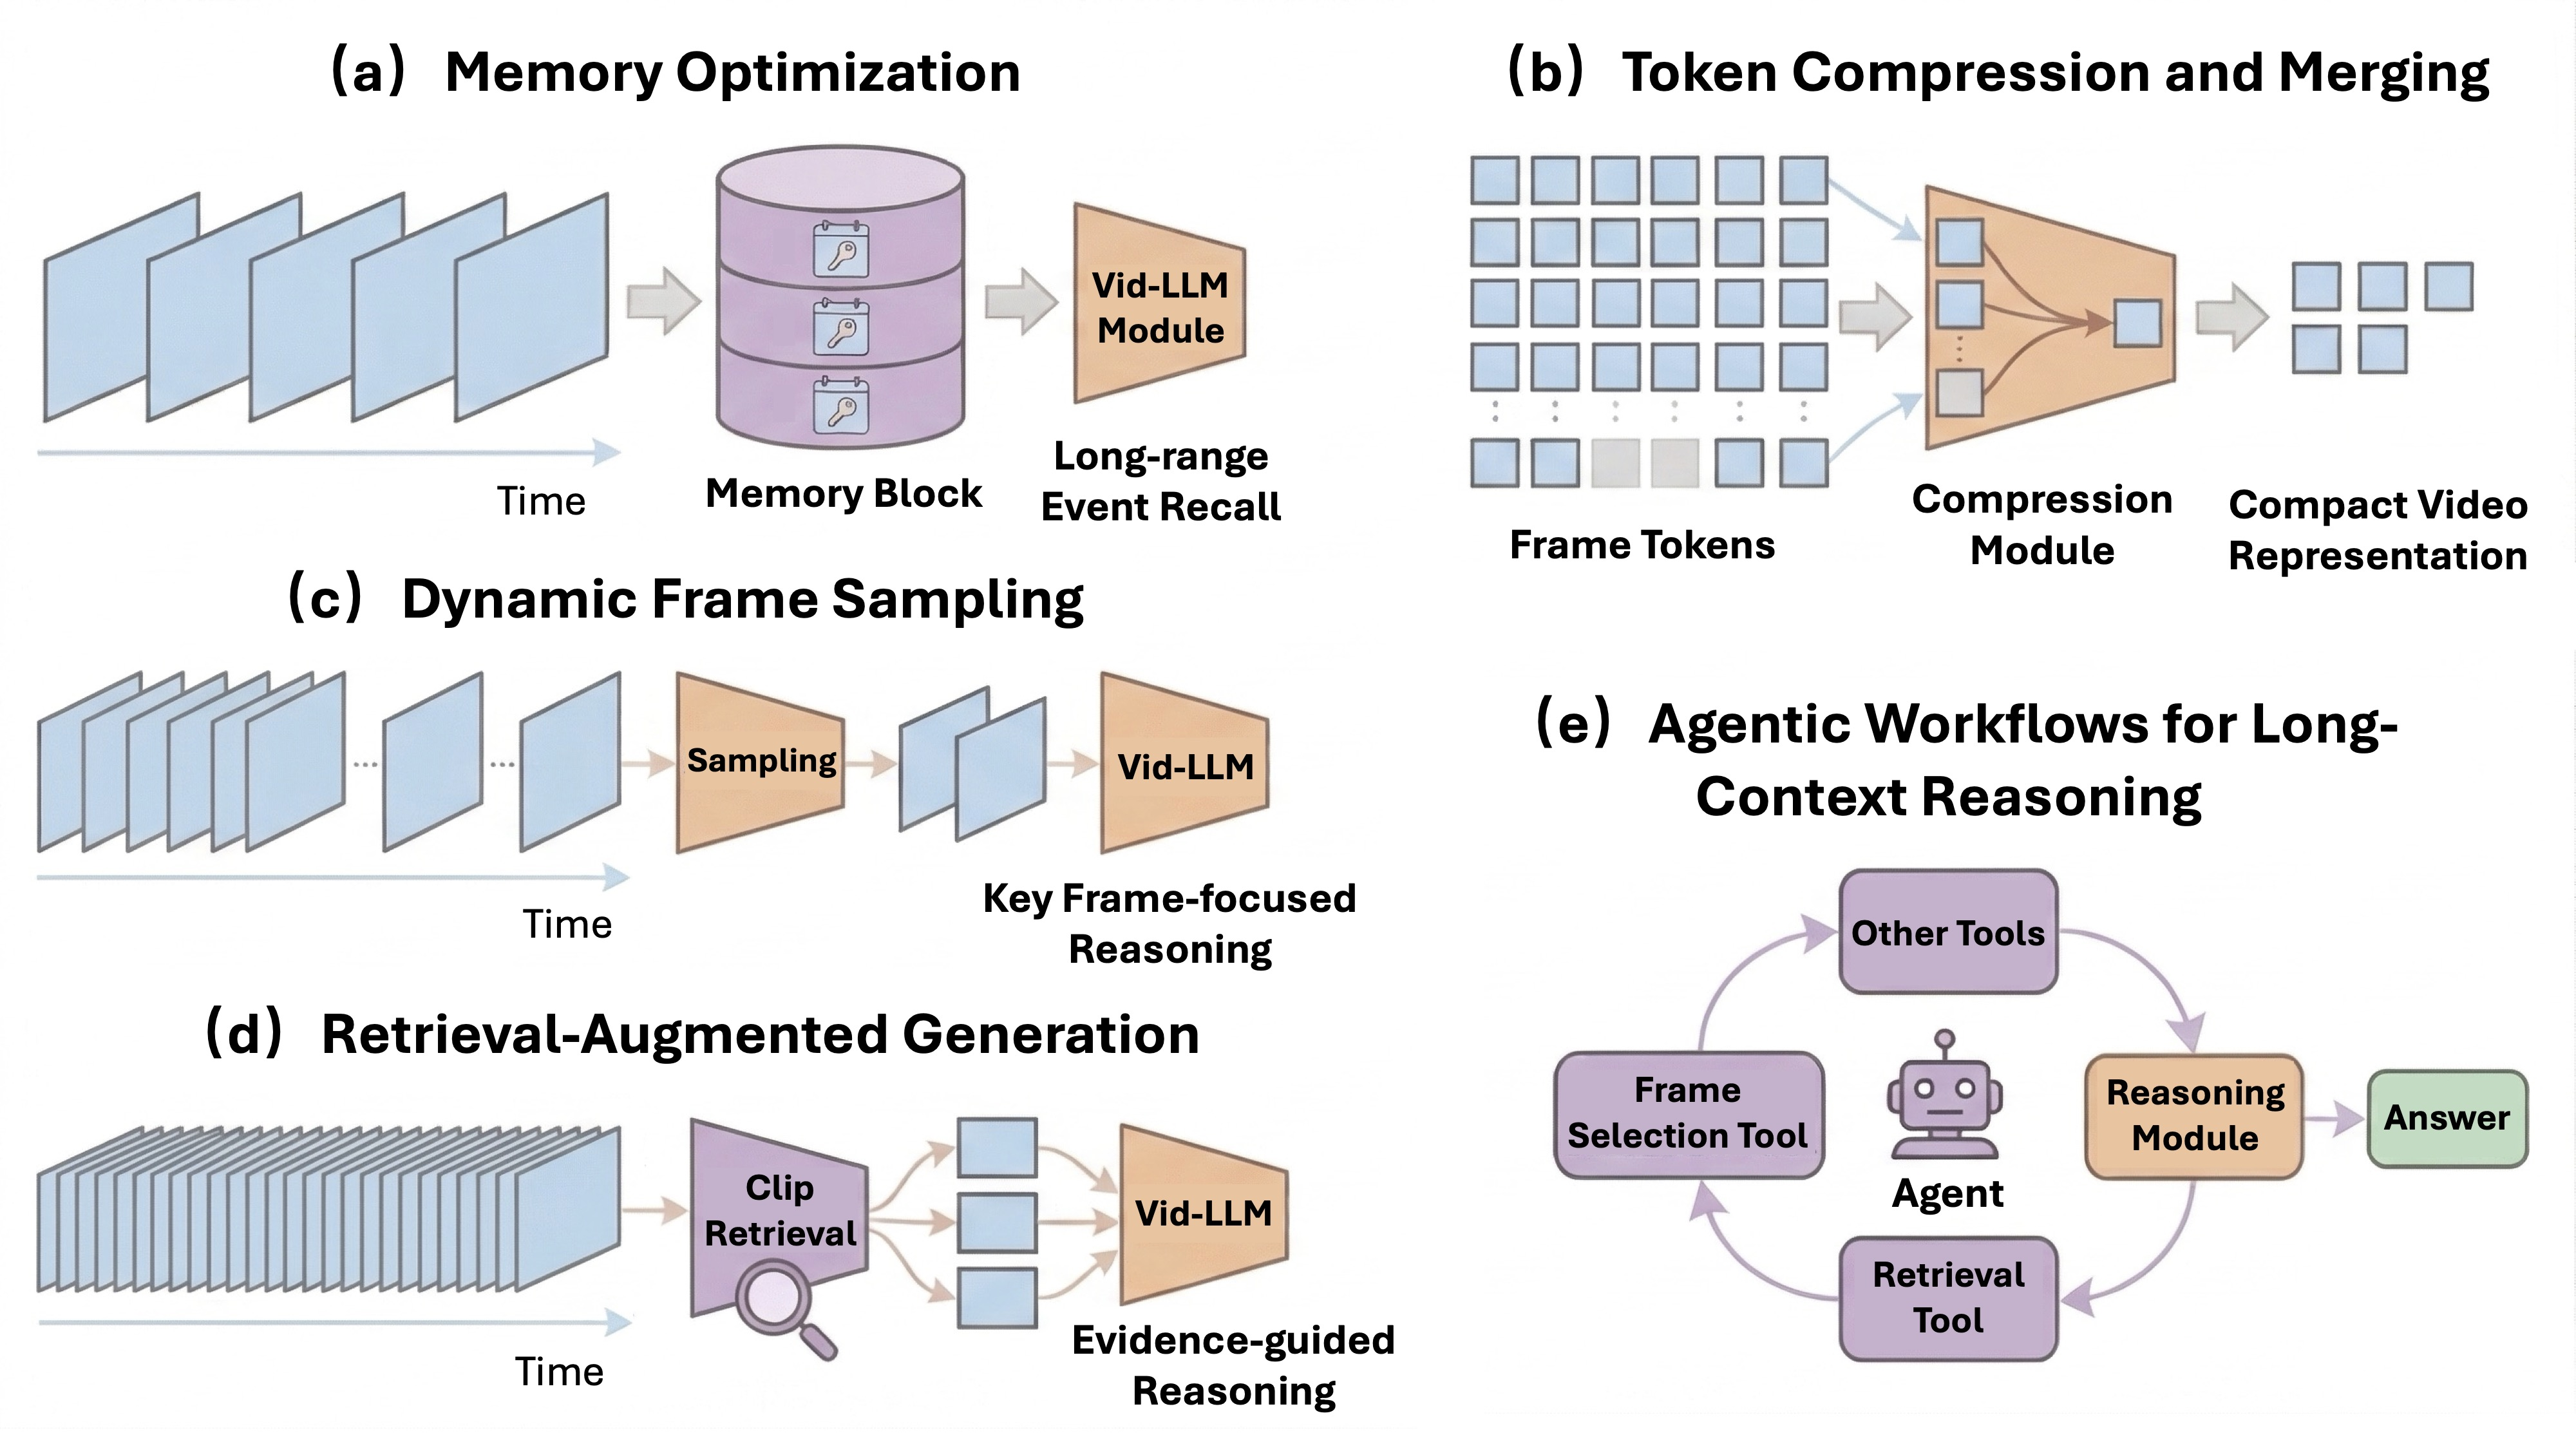
\includegraphics[width=0.95\linewidth]{figure/long_context_hallucination_mitigation.pdf}
  \caption{Illustration of representative methods for mitigating long-context video understanding hallucinations in Vid-LLMs. Each panel depicts a representative strategy corresponding to one category discussed in this subsection, including memory optimization, token compression and merging, dynamic frame sampling, retrieval-augmented generation, and agentic workflows for long-context reasoning.}
  \vspace{-3mm}
\label{fig:mitigation_long_context_hallucination}
\end{figure}

As we've mentioned before, long-context video understanding poses a fundamental challenge because exhaustive frame processing is computationally infeasible, so models rely on aggressive sampling, compression, or memory mechanisms. Hallucinations arise from failures to retrieve, retain, or attend to temporally relevant evidence. We break corresponding mitigation techniques into five subcategories: (i) \emph{memory optimization}; (ii) \emph{token compression and merging}; (iii) \emph{dynamic frame sampling}; (iv) \emph{retrieval augmented generation}; and (v) \emph{agentic workflows for long-context reasoning}.

\paragraph{Memory Optimization}

%Naive approaches that process all frames simultaneously exceed context window limits, while aggressive compression erases fine-grained details. 
%Memory optimization techniques maintain external memory banks or restructure the Key-Value (KV) cache to selectively preserve information.

Early work by \citet{Song2023MovieChatFD} introduced a training-free framework combining a memory buffer with merge-based consolidation, but non-learnable frame merging caused over-smoothing in long videos. VideoLLaMB~\citep{Wang2024VideoLLaMBLV} addresses this with recurrent memory bridges, which are learnable memory tokens within bridge layers, alongside a SceneTiling algorithm for semantic video segmentation, ensuring memories respect scene structure rather than arbitrary chunk boundaries. On NIAVH, VideoLLaMB substantially outperformed MA-LMM~\citep{He2024MALMMML}. A concurrent variant~\citep{Wang2024VideoLLaMBLS} refined this for streaming with linearly scaling recurrent memory caches.

Subsequent work shifted toward human-inspired and online memory mechanisms. Flash-VStream~\citep{Zhang2024FlashVStreamMR} introduced a Spatial-Temporal-Abstract-Retrieved (STAR) memory that dynamically compresses visual information online, achieving real-time inference with lower VRAM. An enhanced version~\citep{Zhang2025FlashVStreamER} decomposed memory into Context Synopsis Memory for temporal aggregation and Detail Augmentation Memory for spatial detail, enabling sub-second responses. It effectively addresses hallucination that arise when coarse narrative state and local visual detail are compressed. $\infty$-Video~\citep{Santos2025VideoAT} augments video Q-formers with continuous-time long-term memory consolidation based on a Gibbs density function, dynamically allocating higher memory granularity to relevant segments, though fine-grained temporal reasoning remains limited when sampling is coarse.

Video-SALMONN S~\citep{Sun2025videoSALMONNSS} replaces token merging with a test-time training layer using Hessian-free optimization to continually update memory representations, processing over one million tokens with fixed memory overhead at approximately 14\% additional computational cost. VideoMem~\citep{Jin2025VideoMemEU} addresses the rigidity of static memory with adaptive memory management trained via Progressive Grouped Relative Policy Optimization (PRPO) with Temporal Cascading Rewards, achieving a $3.1\times$ training speedup. The key insight is: long-context faithfulness depends less on stored tokens than on learning when to retain, rewrite, or discard them.

A parallel line of work targets KV cache compression for streaming. \citet{Yang2025StreamMemQK} introduced query-agnostic KV cache compression with fixed memory footprint, while \citet{Chen2025StreamKVSV} replaced uniform segmentation with dynamic semantic partitioning. \citet{Xu2025StreamingVLMRU} aligned training with streaming inference via overlapped short-chunk attention, achieving competitive performance against GPT-4o mini on infinite-stream evaluation. \citet{Chen2025ScalingRT} developed MR-SP to scale RL training to hour-long videos on a single A100 node via sequence parallelism with cached video embeddings.

Additional strategies include multi-stage long-context training curricula~\citep{Xue2024LongVILASL}, hybrid Mamba-Transformer architectures for linear-complexity processing~\citep{Ren2025VambaUH}, task-aware KV sparsification~\citep{Qin2025TaskAwareKC, Qin2025VideoXL2TV}, and agentic frameworks with adaptive token selection~\citep{Yang2025StreamAgentTA}. The central trade-off remains between memory footprint and retrieval fidelity: aggressive compression risks losing transient events critical for fine-grained reasoning, while richer memory representations undermine real-time applicability.

\paragraph{Token Compression and Merging Strategies}

Token compression reduces representation size by fusing or aggregating visual tokens after encoding. The difficulty is that naive pooling often destroys temporal order, object identity, and scene transitions, which really matter for faithful reasoning.

LongVLM~\citep{Weng2024LongVLMEL} decomposes long videos into segments and applies hierarchical token merging, reducing token counts by roughly two orders of magnitude, but its fixed compression ratio limits adaptability. Dynamic-VLM~\citep{Wang2024DynamicVLMSD} adaptively allocates between 16 and 576 tokens per frame based on video length, substantially improving over LLaVA-OneVision but remaining constrained by a fixed 12K token budget. ReTaKe~\citep{Wang2024ReTaKeRT} jointly reduces temporal and knowledge redundancies through DPSelect for keyframe selection and PivotKV for KV cache compression. It outperformes MovieChat by 3--5\% though degrading on fine-grained tasks such as Needle QA.

Video-XL~\citep{Shu2024VideoXLEV} leverages LLM attention sparsity through Visual Summarization Tokens that adjust compression granularity based on information density. \citet{Wei2024VisualCW} adapt YaRN position embedding extension to visual tokens with progressive pooling, reducing memory by approximately 45\% without retraining. BIMBA~\citep{Islam2025BIMBASC} is the first SSM-based token compression approach, which uses bidirectional selective-scan at $O(N)$ complexity and compressing tokens by 16 times. CrossLMM~\citep{Yan2025CrossLMMDL} decouples visual token processing from the LLM through dual cross-attention, producing text-conditioned compressed representations with sub-linear memory growth. \citet{Dahal2025POVQAPV} combine temporal pooling with DPO, compressing video into a single visual token per second with a 23 times token reduction, though reliability depends on subtitle quality.

\citet{Liu2025VideoXLProRT} introduced reconstructive token compression extending processing to over 8,000 frames while maintaining near-perfect Needle-in-a-Haystack accuracy. This work demonstrates that reconstructive compression preserves semantics better than pure sparsification. \citet{Jiang2025TokenEfficientLV} insert a Mamba-based temporal encoder between image encoder and LLM, showing compression can be built into the sequence processor itself. Complementary strategies include hierarchical caching for streaming~\citep{Wang2025AcceleratingSV}, thumbnail-and-sampling schemes~\citep{Qu2024TSLLaVACV}, and strictly causal two-stage compression~\citep{Chen2025StreamingTOMST}. Token compression is better suited than dynamic sampling when broad temporal coverage must be preserved, but risks semantic averaging where distinct events collapse into a single token.

\paragraph{Dynamic Frame Sampling}

Dynamic frame sampling reduces information overload at the input stage by selecting or filtering frames based on semantic relevance or information density, thus preventing redundancy-induced fabrication before tokens enter the model.

The LIVE framework~\citep{Chen2024VideoLLMonlineOV} introduced Streaming EOS prediction for streaming dialogue, dynamically determining when to respond or remain silent. However, its single CLS token per frame limits spatial understanding. VideoLLM-MoD~\citep{Wu2024VideoLLMMoDEV} introduces a Mixture-of-Depths strategy that selects the top-$k$ most informative vision tokens per frame while routing others through residual connections, reducing FLOPs by 42\% and supporting $1.7\times$ longer context windows. \citet{Sun2024HallucinationMP} combine CLIP-score-guided frame sampling with question-injected visual features, achieving a hallucination rate reduced by over 24\% relative to MovieChat~\citep{Song2023MovieChatFD}. It comes from the key insight that relevance should be defined with respect to the question, not only video salience. SEAL~\citep{Wang2024SEALSA} decomposes long videos into compact scene, object, and action tokens with an Attention Learning module maximizing query relevance and token diversity.

\citet{Sun2025FromFT} extended keyframe extraction to temporally coherent key clips with adaptive resolution, outperforming frame-level baselines on Video-MME and MLVU~\citep{zhou2025mlvu}. \citet{Yao2025KframesSA} reformulated keyframe selection as clip-to-frame prediction preserving scene continuity. \citet{Xu2025EventSTUEE} leveraged event-camera density for coarse-to-fine redundancy removal at lower cost. \citet{Chasmai2025MomentSI} introduced moment sampling through a pre-trained moment retrieval model, yielding consistent gains across four long-form VideoQA benchmarks. \citet{Ok2025DoVL} showed that vision encoder confidence scores do not correlate with downstream performance and that up to 50\% of frames can be removed without significant degradation, motivating segmentation-area-based selection as a more robust alternative.

The design space continues to grow: hierarchical visual retrieval~\citep{Gao2025APVRHL}, RL-based temporal sampling~\citep{Tang2025TSPOTS}, DPP-driven diversity-aware selection~\citep{Wang2025LASTLT}, adaptive frame importance prediction~\citep{Li2025FrameOracleLW}, differentiable selection policies~\citep{Buch2025FlexibleFS}, iterative frame spotlighting~\citep{He2025FrameThinkerLT}, and training-free query-aware sampling~\citep{Liu2025BOLTBL}. Dynamic sampling is most effective when redundancy is high and target evidence is localized; it is less effective when essential information is temporally dispersed or only identifiable after deeper reasoning. %The unresolved tension is between selection accuracy and end-to-end trainability.

\paragraph{Retrieval-Augmented Generation for Long Videos}

Retrieval-augmented generation (RAG) treats the video as a searchable knowledge base, extracting only query-relevant segments. This approach is especially effective when only a small fraction of a long video is relevant.

Naive RAG strategies segment videos mechanically into short clips and retrieve them independently, but they disrupt temporal continuity. Vgent~\citep{Shen2025VgentGR} addresses this with a graph-based framework modeling clips as nodes interconnected by shared entities, outperforming naive RAG by 8.6\% on MLVU~\citep{zhou2025mlvu}. MemVid~\citep{Yuan2025MemoryenhancedRA} maintains a key-value cache for holistic video memorization with generative context-aware query expansion operating directly on video content, reducing contradictions by 8.7\% with lower GPU memory than Video-XL~\citep{shu2025video}. These methods employ retrievals that apply uniform effort regardless of query complexity.

AdaVideoRAG~\citep{Xue2025AdaVideoRAGOA} classifies query intent and dynamically routes questions through hierarchical retrieval paths, from direct inference for simple queries to graph-based retrieval for complex multi-hop reasoning. SceneRAG~\citep{Zeng2025SceneRAGSR} segments videos into narrative-consistent scenes using ASR transcripts and temporal metadata for dynamic knowledge graph construction, since retrieval quality depends on whether indexed units correspond to meaningful event boundaries. Clearly, reliance on ASR quality limits its effectiveness on videos with no or sparse dialogue.

\citet{Ranasinghe2024UnderstandingLV} show that explicit entities serve as better indexing anchors than redundant captions, outperforming LLoVi~\citep{Zhang2023ASL}. \citet{Goulas2024VidCtxCV} replace LLoVi's joint caption processing with a linear-complexity frame-wise approach. \citet{Ma2024DrVideoDR} reformulate long video understanding as document retrieval with multi-stage agent interaction. \citet{Luo2024VideoRAGVR} propose a training-free framework replacing redundant visual tokens with retrieved auxiliary texts (OCR, ASR, object detection), demonstrating that auxiliary text retrieval can be more efficient than additional visual tokens~\citep{Fan2024VideoAgentAM}. Additional efforts decompose long videos into short-term captions for LLM-based reasoning~\citep{Ataallah2024GoldfishVU}. Retrieval-based methods shift complexity from sequence length to indexing quality, but retrieval errors are often unrecoverable, so recent systems increasingly combine retrieval with memory, graph structure, or adaptive routing.

\paragraph{Agentic Workflows for Long-Context Reasoning}

Agentic workflows turn video understanding into a multi-step process of planning, searching, observing, verifying, and revising. %It is a natural response when relevant evidence is sparse, distributed, or uncertain.

\citet{Zhang2025DeepVD} framed long-video understanding as autonomous tool-using search over global, clip-level, and frame-level retrieval. It is a shifte from passive ingestion to active evidence seeking. \citet{Wang2025ActiveVP} replaced caption-heavy preprocessing with direct pixel-level evidence extraction through a plan-observe-reflect loop, reducing token usage.

Several methods strengthen the agentic loop: \citet{Li2025PerceiveRA} leverage multi-granular clue exploration with verification-enhanced reflection; \citet{Dong2025SeeWY} let the model identify reasoning gaps and request targeted visual evidence; VideoLucy~\citep{Zuo2025VideoLucyDM} adds hierarchical memory and backtracking; VideoARM~\citep{Yin2025VideoARMAR} integrates observe-think-act-memorize cycles with hierarchical multimodal memory; and GCAgent~\citep{Yeo2025GCAgentLU} constructs schematic and episodic memory before answering to prevent event merging.

The literature also has works employing collaborative or uncertainty-aware reasoning. LVAgent~\citep{Chen2025LVAgentLV} distributes tasks across multiple specialized Vid-LLM agents. VideoAgent2~\citep{Zhi2025VideoAgent2ET} leverages uncertainty-aware CoT to trigger plan adjustment without heavy external pipelines. TimeSearch~\citep{Pan2025TimeSearchRAT} learns adaptive temporal exploration rather than relying on hand-designed policies, while MR.~Video~\citep{Pang2025MRV} addresses multi-round exploration bottlenecks through a MapReduce-style design analyzing short clips in parallel.

Agentic workflows are especically useful when evidence is sparse or requires iterative disambiguation, while they also introduce latency, planning instability, and possible error propagation. Many successful agentic systems depend on the same components discussed above: retrieval to narrow search, memory to preserve discoveries, and compression to keep iterative inference tractable.

\textbf{Summary.} Long-context hallucination mitigation has evolved from static compression into adaptive systems deciding what to store, process, retrieve, or revisit. Memory methods excel when continuity matters but require robust retention policies. Sampling and compression improve efficiency but risk removing decisive evidence. Retrieval-augmented methods scale well but remain affected by retrieval misses. Agentic workflows offer the greatest flexibility and quality at the cost of latency, cost, and complexity. %A promising direction is integrating these paradigms into unified pipelines coupling adaptive memory, structure-aware retrieval, and verification-driven exploration.


\subsection{Object Hallucination Mitigation}
\label{subsec:object-hallucination-mitigation}

\begin{figure}[t]
  \centering
  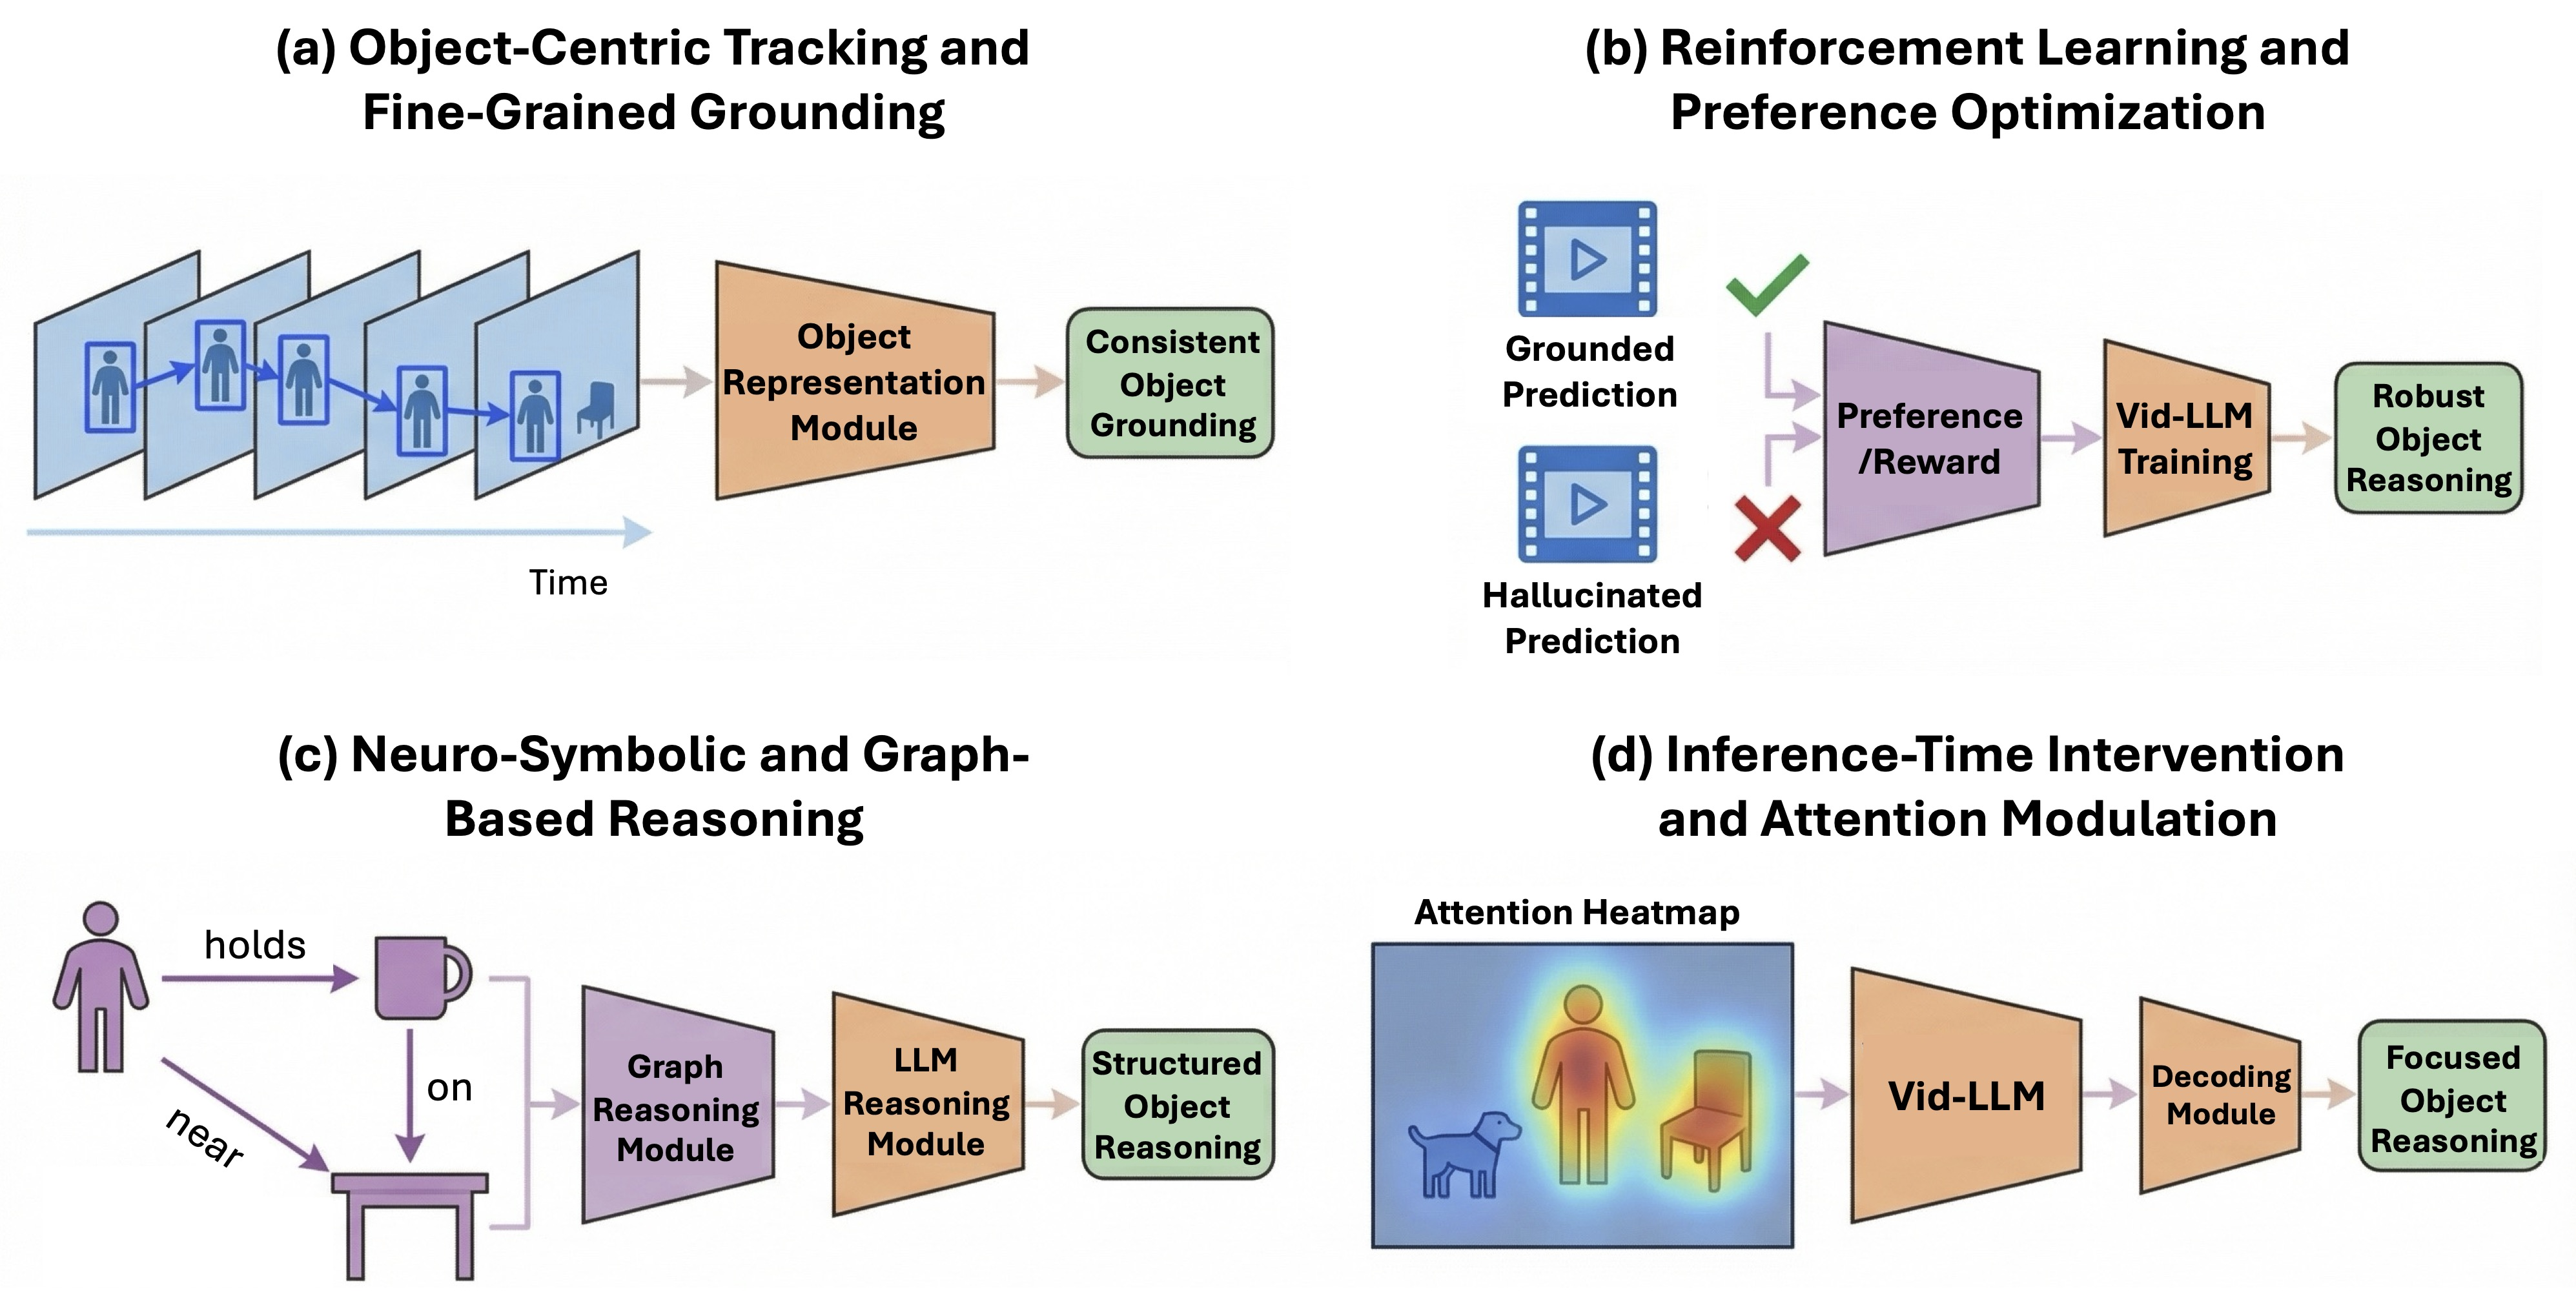
\includegraphics[width=0.95\linewidth]{figure/object_hallucination_mitigation.pdf}
  \caption{Overview of representative strategies for mitigating object hallucinations in Vid-LLMs. The panels illustrate four major solution paradigms discussed in this subsection: (a) object-centric tracking and fine-grained grounding for maintaining consistent object representations; (b) reinforcement learning and preference optimization that penalize unsupported object predictions during training; (c) neuro-symbolic and graph-based reasoning that structures entities and relations for grounded reasoning; and (d) inference-time intervention and attention modulation that dynamically steers the model toward visually grounded evidence.}
  \vspace{-3mm}
\label{fig:mitigation_object_hallucination}
\end{figure}

Object hallucination arises from failures to consistently aggregate object evidence across time, due to motion, occlusion, and appearance variation, which make object perception more complex than in static images. We break the solutions into four subcategories: (i) \emph{object-centric tracking and fine-grained grounding}; (ii) \emph{reinforcement learning and preference optimization}; (iii) \emph{neuro-symbolic and graph-based reasoning}; and (iv) \emph{inference-time intervention and attention modulation}.

\paragraph{Object-Centric Tracking and Fine-Grained Grounding}

The most direct remedy is to force models to explicitly localize, track, and reason about specific entities rather than relying on holistic scene representations. VideoGLaMM~\citep{Munasinghe2024VideoGLaMMA} introduces a dual vision encoder (spatial and temporal) with a spatiotemporal decoder for precise mask generation, substantially improving interrogative mIoU on VidSTG~\citep{zhang2020does} over PG-Video-LLaVA~\citep{Munasinghe2023PGVideoLLaVAPG}. Mask supervision forces the model to maintain correspondence between words and localized visual evidence. On the other hand, producing pixel-level masks is expensive, and its consistency struggles with objects of varying granularity across long sequences.

ObjectMLLM~\citep{Tang2025HowCO} encodes bounding boxes and labels as quantized text tokens, nearly doubling accuracy on CLEVRER-MC~\citep{yi2019clevrer} when augmenting VideoLLaMA~2~\citep{Cheng2024VideoLLaMA2A}. RGA3~\citep{Wang2025ObjectcentricVQ} supports arbitrary visual prompts, including masks, bounding boxes, arrows, points, and scribbles, as both input and output, with a Spatial-Temporal Overlay Module propagating prompts across frames, reducing hallucination rates by approximately 10\% over VideoRefer~\citep{Yuan2024VideoReferSA}. Many hallucinations arise not from failure to detect an object once but from failure to maintain its identity over time.

\citet{Gu2025KnowingYT} introduced text-guided temporal sampling and attribute-aware spatial activation, improving grounding on HCSTVG-v1~\citep{tang2021human} over TubeDETR~\citep{Wasim2023VideoGroundingDINOTO}. \citet{Gao202511} coupled an MLLM with an open-vocabulary detector through a reference-semantic token, boosting m\_vIoU from 8.2 to 36.2 on HC-STVG v1. \citet{Kazakos2025LargescalePF} extended grounded captioning to video with spatio-temporal adapters and a temporal objectness head, yielding 20 CIDEr points on iGround~\citep{kazakos2025large}. It demonstrates that object-faithful generation benefits from temporal consistency constraints, not only spatial localization.

Complementary works include region-level token marks~\citep{Heo2025OmniRGPTUI}, semantically decoupled slots~\citep{Xu2024SlotVLMSS}, grid-based local-global transcription~\citep{Chowdhury2025GridLOGATGB}, intention-oriented box adapters~\citep{Qiu2025IntentVCNetBS}, open-vocabulary detection for validation~\citep{Montes2025ViQAgentZV}, tokenized object dynamics~\citep{Feng2024VideoOrionTO}, and fused multi-encoder architectures~\citep{Chung2025UnifyingSV}. The consistent principle is that anchoring outputs to verifiable spatiotemporal evidence suppresses perceptual hallucinations. On the other hand, fine-grained grounding often depends on external detectors, dense supervision, or expensive token budgets, which are costly for long, cluttered videos.

\paragraph{Reinforcement Learning and Preference Optimization}

As discussed, preference optimization reshapes the output distribution by penalizing hallucinated entities, attributes, and spatial relations. VideoSAVi~\citep{Kulkarni2024VideoSAViSV} pioneered self-aligned Vid-LLM training: a self-critiquing mechanism identifies reasoning errors and generates on-policy preference pairs for DPO without external supervision, yielding gains on MVBench~\citep{li2024mvbench} and EgoSchema~\citep{mangalam2023egoschema}. The model is trained to distinguish visually faithful descriptions from unsupported ones. Its iterative self-play is relatively computationally expensive.

VistaDPO~\citep{Huang2025VistaDPOVH} introduced hierarchical spatial-temporal alignment at three levels: instance semantics, temporal events, and fine-grained spatial-object grounding. It applies token-level optimization via sequential KL divergence, outperforming coarse baselines on VideoHallucer~\citep{wang2024videohallucer} and EventHallusion~\citep{Zhang2024EventHallusionDE}. PaMi-VDPO~\citep{Ding2025PaMiVDPOMV} eliminates offline data dependence by dynamically generating rejected samples through video augmentations, achieving competitive performance with only 10k samples. VideoPASTA~\citep{Kulkarni2025VideoPASTA7P} constructs targeted adversarial preference pairs contrasting dense and sparse temporal sampling, demonstrating that careful augmentation can rival methods requiring far larger preference-labeled datasets.

Oracle-RLAIF~\citep{Shi2025OracleRLAIFAI} replaces trained scalar reward models with an Oracle ranker providing ordinal feedback via GRPO$_{\text{rank}}$. It reports outperforming prior RLAIF approaches~\citep{Ahn2024TuningLM}. ViSS-R1~\citep{Fang2025ViSSR1SR} shows that self-supervised pretext-task rewards can complement preference-based objectives without architectural modifications. Additional works include QA-driven reward signals~\citep{Liu2024QAVidCapEV}, self-consistency-based preference pair construction~\citep{Dang2025SynPOSD}, and detection-and-tracking pipelines with RL policies to minimize false positive object mentions~\citep{Shankar2025AnEV}.

Preference-based methods are architecture-agnostic. They shape outputs indirectly: if the underlying representation lacks reliable object evidence, optimization may reduce blatant hallucinations but fail on rare objects, heavy occlusion, or fine-grained spatial distinctions. These methods need to be paired with representations that already expose object structure.

\paragraph{Neuro-Symbolic and Graph-Based Reasoning}

Neuro-symbolic and graph-based methods impose structural constraints by converting unstructured video into explicit relational graphs enforcing verifiable reasoning over entities. ReGR~\citep{Wang2023ReGRRG} introduces a dual-graph architecture: a Spatiotemporal Graph Attention Network captures object dynamics, while a Multi-Relation Graph Attention Network encodes fine-grained interactions, with question-guided filtering to suppress irrelevant features. This improved accuracy on TGIF-QA~\citep{jang2017tgif} FrameQA but degraded on longer videos requiring complex temporal reasoning.

LGQAVE~\citep{Rongali2024FoundationMA} constructs dynamic spatial object graphs conditioned on masked question embeddings via a Question-aware Dynamic Graph Transformer, leveraging MiniGPT-4 for visual grounding. NExT-QA~\citep{xiao2021next} accuracy rose from 53.68\% to 66.69\%, and MSRVTT-QA~\citep{xu2016msr-vtt} from 39.70\% to 63.43\%, surpassing CoVGT~\citep{Xiao2023ContrastiveVQ}, which lacks question-specific conditioning. The shift from static to question-conditioned graphs is important since some object hallucinations are due to selecting the wrong subset of entities for the question at hand. However, computational overhead (289 GFlops) and reliance on MiniGPT-4 limit scalability beyond 600 frames.

\citet{Dai2025TowardsFV} integrated an explicit scene graph predictor, improving MOMA-QA accuracy from 76.62\% to 79.66\% over SeViLA~\citep{Yu2023SelfChainedIM}. Complementary efforts encode textual scene graph sequences~\citep{Linok2025DyGEncEA}, leverage dual and heterogeneous graphs~\citep{Liang2025LeveragingSR}, and inject scene graphs into Vid-LLM prompts. What is central in this line of work is that hallucination is reduced by making object claims pass through a structured reasoning bottleneck. 

\paragraph{Inference-Time Intervention and Attention Modulation}

Inference-time interventions redirect attention toward task-relevant visual evidence during generation, offering a training-free alternative. SFA (Scan, Focus, and Amplify)~\citep{He2025SFASF} integrates an external Video Text Spotting model with a three-stage pipeline: candidate text region detection, adaptive windowing with multimodal scoring, and region enhancement. SFA achieved up to 45.80\% improvement over prior methods, including a 10.85\% accuracy gain over Qwen2.5-VL-7B on RoadTextVQA~\citep{tom2023reading}, surpassing GAT~\citep{Zhang2025GatherAT}. Instead of trusting learned attention maps, it explicitly re-centers decoding on localized visual-textual content, though effectiveness is bounded by the text spotting model's accuracy.

\citet{Jung2023RetrievalaugmentedVE} augmented visual frame representations with externally retrieved textual descriptions, reducing hallucinated object mentions in dense captioning.
Inference-time interventions offer zero training cost, modularity, and compatibility with arbitrary base models, but remain narrowly scoped. Their success hinges on reliably identifying the right evidence.

\textbf{Summary.} Now let us compare the subcategories. Object-centric grounding is very direct and faithful, also realatively expensive. Preference optimization is more modular but cannot compensate for weak visual representations. Graph-based reasoning improves interpretability but relies on accurate scene parsing. Inference-time intervention is training-free and relatively narrow-scoped. 
%A promising direction combines structured grounding with lightweight preference signals and inference-time attention steering.


\subsection{Causal and Reasoning Hallucination Mitigation}
\label{subsec:reasoning-hallucination-mitigation}

\begin{figure}[t]
  \centering
  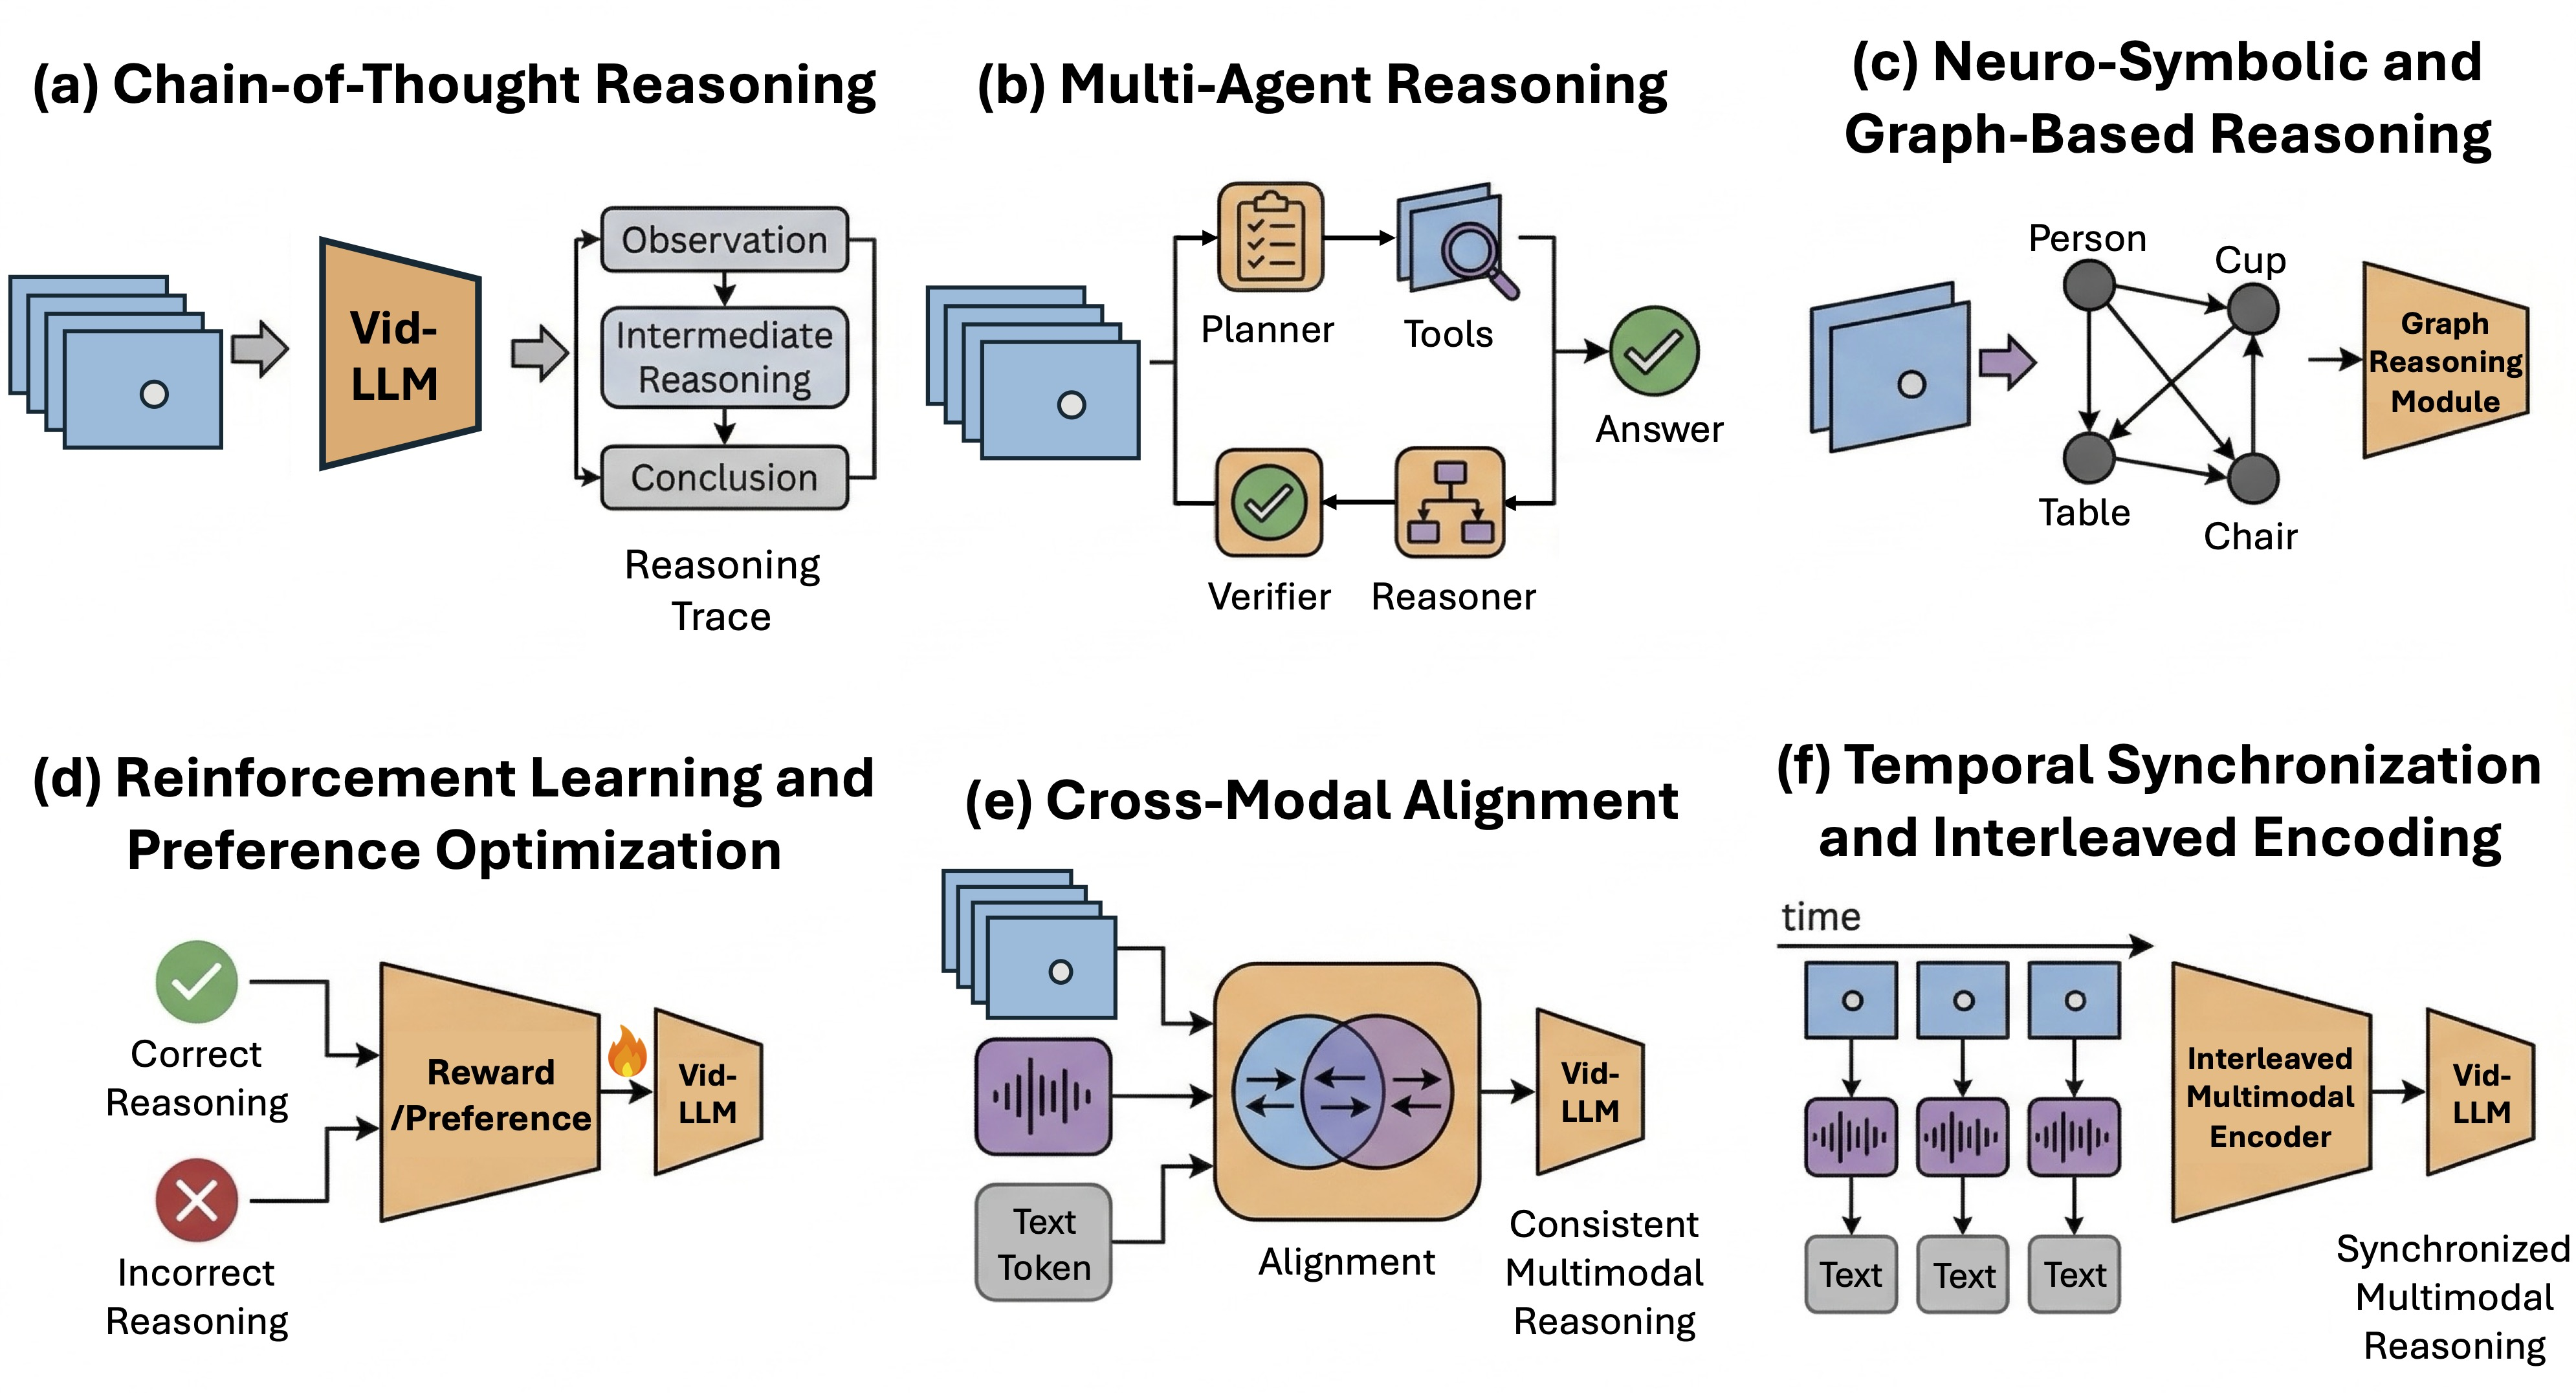
\includegraphics[width=0.95\linewidth]{figure/reasoning_and_cross_modal_hallucination_mitigation.pdf}
  \caption{Representative mechanisms for mitigating causal and reasoning, and cross-modal hallucinations in Vid-LLMs. Panels (a)--(d) illustrate reasoning-level mitigation strategies discussed in Section~\ref{subsec:reasoning-hallucination-mitigation}, including chain-of-thought reasoning, multi-agent reasoning, neuro-symbolic and graph-based reasoning, and reinforcement learning with preference optimization. Panels (e) and (f) present representative approaches for cross-modal hallucination mitigation described in Section~\ref{subsec:cross-modal-hallucination-mitigation}, including cross-modal alignment and temporal synchronization with interleaved multimodal encoding.}
  \vspace{-3mm}
\label{fig:mitigation_reasoning_and_cross_modal_hallucination}
\end{figure}

Causal and reasoning hallucination mitigation addresses failures where models generate unsupported causal relations, intentions, or abstract conclusions. We subcategorize its mitigation techniques as (i) \emph{reinforcement learning and preference optimization}; (ii) \emph{neuro-symbolic and graph-based reasoning}; (iii) \emph{chain-of-thought reasoning}; and (iv) \emph{multi-agent reasoning frameworks}.

\paragraph{Reinforcement Learning and Preference Optimization}

RL and preference optimization penalize logically inconsistent or visually ungrounded reasoning traces during post-training. Video-R1~\citep{Feng2025VideoR1RV} established the viability of RLVR for video reasoning but also exposed three challenges: holistic captions erasing temporal structure, training data solvable from textual priors alone, and CoT traces grounded in commonsense rather than visual evidence. Subsequent work has systematically addressed these limitation.

VideoRFT~\citep{Wang2025VideoRFTIV} introduces a cross-modal CoT refinement stage where an MLLM revises initial reasoning by re-examining the video, with a semantic-consistency reward enforcing visual-textual alignment, yielding consistent gains over Video-R1~\citep{Feng2025VideoR1RV}. Video-R2~\citep{Maaz2025VideoR2RC} adds a Temporal Alignment Reward and consistency gating that link reasoning trace claims to timestamps and the final answer, improving think-answer consistency across eleven benchmarks. %causal hallucinations often occur when one unsupported intermediate step contaminates an otherwise plausible explanation. 
Addressing \emph{visual thinking drift}, \citet{Luo2025WhenTD} proposed the Visual Evidence Reward where an auxiliary judge evaluates whether intermediate steps reference verifiable visual evidence, achieving up to 9.0\% gains on TempCompass.

Standard binary rewards cannot distinguish partially correct reasoning from fabricated chains. TW-GRPO~\citep{Dang2025ReinforcingVR} enables finer-grained credit assignment through token-level importance weighting based on information entropy with multi-level soft rewards, achieving 18.8\% improvement on CLEVRER~\citep{yi2019clevrer} over Video-R1. VerIPO~\citep{Li2025VerIPOCL} employs a Rollout-Aware Verifier within an iterative GRPO-Verifier-DPO loop, making DPO training $7\times$ faster than GRPO. Reflection-V~\citep{Jian2025LookAT} tackles visual attention decay in long reasoning chains through cold-start initialization with visual reflection data and a visual attention-based reward.

ReWatch-R1~\citep{Zhang2025ReWatchR1BC} pairs multi-agent data synthesis simulating re-watching behavior with an Observation and Reasoning reward, reducing text-only solvability from 68.9\% to 29.4\%. VidBridge-R1~\citep{Chen2025VidBridgeR1BQ} identifies a conflict between convergent QA and divergent captioning objectives, introducing intermediate proxy tasks (e.g., masked event inference and segment isolation) while eliminating the supervised fine-tuning stage. Conan~\citep{Ouyang2025ConanPL} combines multi-scale frame categorization with difficulty-aware progressive training. It reports surpassing Video-R1 by 10\%+ across six multi-step reasoning benchmarks.

ReAgent-V~\citep{Zhou2025ReAgentVAR} shifts optimization to inference time through a modular multi-agent framework generating real-time rewards via Entropy-Calibrated Relevance Scores, achieving improvements with only 45\% of the training data. Complementary efforts include reinforced causal keyframe search~\citep{Zhou2025ReaSonRC}, rank-based RLAIF~\citep{Shi2025OracleRLAIFAI}, and self-training with preference optimization~\citep{Zohar2024VideoSTaRSE}.
From these works, we can observe progression from simple binary outcome rewards toward sophisticated supervision of intermediate reasoning. %Reward design remains fragile for implicit causality, emotion, and long-horizon multi-hop reasoning.

\paragraph{Neuro-Symbolic and Graph-Based Reasoning}

Neuro-symbolic and graph-based approaches address causal hallucinations by constructing explicit structured representations that ground inference in observable entities and relationships. It makes inferential chains auditable by design.

Some hallucinations are confounding problems where the model mistakes correlation for causality. To alleviate this, EIGV~\citep{Li2022EquivariantAI} partitions visual scenes into causal and environment components through a Structural Causal Model, enforcing equivariant and invariant grounding via contrastive learning, improving over invariant-only approaches~\citep{Li2022InvariantGF} on MSVD-QA~\citep{Xu2017VideoQA}.  VCSR~\citep{Wei2023VisualCS} applies causal front-door interventions through a Question-Guided Refiner and Causal Scene Separator, achieving gains on predictive and counterfactual tasks over methods~\citep{Liu2022CrossModalCR} that neglected temporal causal refinement.
\citet{Lyu2023SemanticAwareDR} leverage Semantic Role Labeling (SRL) to guide multi-step retrospective-prospective reasoning, dynamically attending to different SRL arguments and selecting relevant frames. This substantially improves TrafficQA~\citep{xu2021sutd} accuracy over prior graph-convolutional methods, though reliance on SRL parser quality limits generality.

GHR-VQA~\citep{Brilli2025GHRVQAGH} constructs human-rooted video-level graphs with hierarchical conditional relational networks, efficiently modeling human-object interactions though limited to single-actor scenes. \citet{Tang2024SpatioTemporalGC} extend with dynamic graph convolution transformers. Broader explorations include entailment-tree frameworks~\citep{Sanders2024TVTREESME}, scene-graph and knowledge-graph fusion~\citep{Taluzzi2025FromPT}, scene graph-guided self-training~\citep{Qiu2024STEPEV}, theory-of-mind reasoning~\citep{Chen2024ThroughTT}, and causal-aware temporal grounding~\citep{Dong2025LeAdQALC}.

The advantages of these methods include transparency and auditable reasoning chains, but they come at the cost of requiring clean scene decomposition, reliable detection and extraction, and accurate parsing. These methods are strongest when the reasoning problem has clear compositional structure and where interpretability is important.

\paragraph{Chain-of-Thought Reasoning}

CoT reasoning decomposes complex inferential tasks into intermediate steps, grounding each logical transition in observable evidence. 
Note that free-form textual CoT (which ignores visual evidence) can actually worsen hallucination here. Only when intermediate reasoning is visually grounded does the CoT reduce hallucination.

ViTCoT~\citep{Zhang2025ViTCoTVI} uses a video-text interleaved paradigm that re-examines key frames at each reasoning step, achieving 5.5\% improvement over baseline CoT. Causal questions often require returning to evidence after a hypothesis is formed. ChainReaction~\citep{Parmar2025ChainReactionCC} tackles causal-why video QA through a modular two-stage architecture: a Causal Chain Extractor generates chains grounded in Structural Causal Models, and a Causal Chain-Driven Answerer derives responses. While outperforming monolithic baselines, approximately 38\% of errors originate from misinterpretation of object roles during chain extraction.

CoT-Vid~\citep{Jin2025VISTAMS} introduces dynamic inference path routing determining whether a question requires multi-step reasoning or direct answering, with video self-consistency verification. This training-free framework outperforms Video-R1 by 9.3\% on EgoSchema~\citep{mangalam2023egoschema}, avoiding unnecessary reasoning cost on simple queries.

\citet{Liu2025CommonsenseVQ} introduce video-grounded entailment tree reasoning. It achieves a competitive performance with $257\times$ fewer parameters than VideoAgent~\citep{Wang2024VideoAgentLV}. \citet{Liang2025ReasVQAAV} refine imperfect MLLM-generated chains via a three-phase filter-and-learn pipeline. \citet{Wang2023VamosVA} replace visual embeddings with text descriptions and a token bottleneck, achieving $5\times$ inference speedup. Other works include perception-to-cognition pipelines~\citep{Fei2024VideoofThoughtSV}, atomic task planning~\citep{Chen2025VQAGuiderGM}, reasoning chain distillation~\citep{Shi2024EnhancingVR}, sub-task-oriented instruction tuning~\citep{Wang2025CoTasksCB}, counterfactual thought chains~\citep{Zhang2025CanVL}, and decomposition-based subquestions~\citep{Kamoto2025DIVEDI}.
From these works we can observe that CoT helps only when the chain remains tethered to visual evidence. % Tighter integration of fine-grained visual grounding within each reasoning step, rather than post hoc frame retrieval, remains an open challenge.

\paragraph{Multi-Agent Reasoning}

Multi-agent frameworks extend CoT to collaborative, iterative processes where specialized agents debate, verify, and refine intermediate inferences, directly targeting error propagation where an early causal misattribution corrupts all downstream conclusions.

MoReVQA~\citep{Min2024MoReVQAEM} decomposed video QA into fixed stages that proved brittle when queries did not conform. CAViAR~\citep{Menon2025CAViARCV} shifts to adaptive, iterative execution: a reasoning agent dynamically composes video-processing modules based on intermediate results, and then a natural-language critic evaluates sampled reasoning traces. CAViAR achieves 77.2\% on LVBench~\citep{wang2025lvbench} versus 48.7\% for direct inference. %, though it struggles with ultra-long videos exceeding one hour.

From different perspectives, \citet{Xie2025TeamOO} orchestrate diverse prompting strategies with an MLLM-based evaluator for compositional and causal reasoning without task-specific training. ReAgent-V~\citep{Zhou2025ReAgentVAR} generates evaluation reports during inference as dynamic rewards, employing reflection across conservative, neutral, and aggressive perspectives. VideoAgent~\citep{Fan2024VideoAgentAM} frames video reasoning as iterative collaboration where specialized agents collaboratively select, analyze, and refine reasoning through reward-driven feedback.

Once again, multi-agent collaboration offers clear advantages in error recovery and reasoning diversity, but also introduces coordination overhead, latency, and reliance on critic agents. This is an active line of research because mitigating causal hallucination require not just a better model but a better reasoning process.

\textbf{Summary.} Now let us compare. RL reshapes model behavior through reward-driven post-training; neuro-symbolic methods make reasoning auditable; CoT externalizes intermediate logic for verification; and multi-agent systems enable procedual error correction. %RL depends on reward function quality; graph-based approaches suffer from brittle dependencies; CoT and multi-agent frameworks incur inference-time cost. 
Clearly, a promising direction is to combine verifier-trained rewards, structured representations, evidence-grounded reasoning traces, and lightweight agentic verification.

\subsection{Cross-Modal Hallucination Mitigation}
\label{subsec:cross-modal-hallucination-mitigation}
Cross-modal hallucination mitigation addresses failures in integrating evidence across visual, audio, and textual modalities. Their mitigation approaches fall into two subcategories: (i) \emph{temporal synchronization and interleaved encoding}; and (ii) \emph{cross-modal alignment and contrastive tuning}.

\paragraph{Temporal Synchronization and Interleaved Encoding}

Fine-grained temporal alignment between audio and visual signals is essential for preventing misattribution of auditory cues. Early Vid-LLMs such as Video-LLaMA~\citep{Zhang2023VideoLLaMAAI} processed modalities through largely independent adapters, resulting in weak audio exploitation. VideoLLaMA~2~\citep{Cheng2024VideoLLaMA2A} replaced this with a Spatial-Temporal Convolution connector employing 3D convolutions and integrated a BEATs audio encoder, improving on EgoSchema but remaining coarse-grained beyond eight frames.

As an explicit temporal encoding method, OMCAT~\citep{Goel2024OMCATOC} introduces Rotary Time Embeddings (RoTE) encoding absolute timestamps as rotation angles into both audio and visual tokens, as many cross-modal hallucinations arise from the model's inability to determine which signal belongs to which moment. OMCAT nearly doubled VideoLLaMA~2's accuracy and outperformed AVicuna~\citep{Shu2023AudioVisualLF}.

Along this direction, Dolphin~\citep{Guo2025AlignedBL} addresses both spatial and temporal dimensions through a multi-scale audio-visual adapter and interleaved temporal merging, reducing hallucination rates by nearly 40\% on speech-aware samples. Temporal synchronization is most effective when paired with source localization. \citet{Chen2025LiveLV} shifted to frame-level alignment through a streaming paradigm densely interleaving ASR word tokens with video frames based on precise timestamps, achieving state-of-the-art real-time commentary with 30$\times$ latency reduction over Vid2Seq~\citep{Yang2023Vid2SeqLP}, though inheriting ASR errors. \citet{Ge2025ARCHunyuanVideo7BSV} augmented captioning models with an auxiliary audio encoder and adaptive duration-based synchronization for multi-granularity temporally grounded captioning.

The central insight of these methods is: cross-modal hallucination often occurs asa sequencing problem rather as a representation problem. Models fail because they fuse modalities too early, too coarsely, or without a reliable notion of event order. A persistent challenge worth noting is how to handle temporally overlapping or weakly correlated audio-visual events.

\paragraph{Cross-Modal Alignment}

While temporal synchronization addresses \emph{when} modalities should be aligned, cross-modal alignment addresses \emph{what} should be aligned by enforcing representational consistency across video, audio, and text feature spaces.

\citet{Yang2024RobustVQ} proposed a self-supervised contrastive regularization framework that contrasts original and perturbed multimodal inputs with temporal order regularization, reducing reliance on superficial question-scene correlations beyond the invariant grounding of \citet{Li2022InvariantGF}. \citet{Bansal2023VideoConRV} leveraged contrast captions with temporal and action perturbations, improving temporal reasoning~\citep{Bagad2023TestOT, Momeni2023VerbsIA}. \citet{Zhao2025CanHC} replaced VideoCon's binary contrastive signal with a self-training hallucination correction objective, outperforming it by up to 17.9\% on VELOCITI~\citep{saravanan2025velociti}.

InternVideo2~\citep{Wang2024InternVideo2SF} introduced a progressive three-stage paradigm unifying masked video modeling, cross-modal contrastive learning across video-audio-speech-text, and next-token prediction within a 6B-parameter model. It goes beyond video-text contrastive scope~\citep{Li2023UnmaskedTT} and achieves retrieval gains on MSR-VTT~\citep{xu2016msr-vtt}. \citet{Li2023ObjectawareAL} introduced object-aware adaptive-positivity contrastive learning aligning question-object and audio-object pairs individually on MUSIC-AVQA~\citep{li2022learning}. Clearly, alignment has become more about constructing a shared multimodal space preserving motion, speech, and semantics. 

In the causal reasoning line of work, \citet{Chen2025CrossmodalCR} formulated a Structural Causal Model for multimodal deconfounding, employing front-door adjustment on visual features and back-door adjustment on linguistic features. Causal alignment is better suited to reducing unfaithful grounding than correlation-based methods alone, since a model may attend to aligned segments that are not the true basis for the answer. This reduced bias-induced errors over data-driven baselines~\citep{Xiao2023CanIT}, demonstrating that causal interventions complement contrastive strategies in weakly supervised settings.

There are also architectural innovations for alignment. \citet{Liu2023VideoTellerEC} proposed a cascaded Q-Former reducing severe hallucination rates from 34\% to 20\% on Video-CSR~\citep{liu2023video}. Additional efforts include mutual knowledge transfer~\citep{Weng2022VisualAL}, bidirectional set-level alignment~\citep{Wang2023LearningGV}, multi-grained correspondence learning~\citep{Wang2024GEXIAGE}, codebook-based discretization~\citep{Zhu2025VTDCLIPVD}, sparse masked pre-training~\citep{Lin2022SMAUGSM}, congruity matching~\citep{Zeng2023TVTSv2LO}, and dual-task representations~\citep{Wang2024DualTaskMR}. The most effective recent methods distinguish themselves by finer control over what is aligned: timestamps, objects, speech spans, event order, or causal evidence.

\textbf{Summary.} In the cross-modality category, temporal synchronization ensures correct chronological pairing, and cross-modal alignment enforces semantic consistency across feature spaces. Synchronization has evolved from independent fusion through timestamp encoding to fine-grained interleaving. Alignment spans contrastive regularization, multimodal pretraining, object-level grounding, and causal deconfounding. Fine-grained methods improve faithfulness but increase cost. Open challenges include robust reasoning over temporally overlapping or weakly correlated events, handling arbitrary modality combinations, and efficient scaling to long-form video.

% \label{sec:suggestion}
% \todo{Finish this section.}
\section{Future Directions}
\label{sec:future_directions}
We have mentioned many open challenges along the way, which limit the reliability of Vid-LLMs in real-world deployment. Here we highlight future directions we believe promising.

\subsection{Benchmarking and Evaluation for Video Hallucination}
Current benchmarks overwhelmingly measure task-level accuracy without disentangling whether strong performance reflects faithful video grounding or fluent confabulation~\citep{Maaz2023VideoChatGPTTD, Zhang2024LLaVAVideoVI}. Actually, a model may achieve highly competitive scores while still fabricating objects, inventing temporal orderings, or hallucinating causal relationships not evident in the video.

Designing benchmarks that directly evaluate hallucination in video understanding is challenging. First, annotations must specify not only what is present but also what is absent, i.e., explicit negative labels for objects, events, or temporal relations that models might plausibly hallucinate. Second, metrics must move beyond binary correctness to measure grounding accuracy, for example, whether each claim is supported by specific visual evidence at the correct temporal location~\citep{Xiao2023CanIT, Guo2024TRACETG}. Analyses on NExT-GQA~\citep{xiao2024can} show that models that achieve nearly 70\% QA accuracy ground their answers in relevant segments only less than 20\% of the time~\citep{Xiao2023CanIT}. Third, without saying, benchmarks must cover diverse temporal scales and hallucination types.
Last but not least, rigorous benchmarks should move evaluation beyond only proxy tasks that may not reflect genuine faithfulness improvements.

\subsection{Out-of-Schema Strategies }
Most mitigation methods assume that encountered entities, actions, and event structures fall within the training distribution~\citep{Maaz2023VideoChatGPTTD, Chen2024ShareGPT4VideoIV}. But real-world videos routinely present novel entities and previously unseen event configurations. When confronted with such new inputs, Vid-LLMs may project unfamiliar percepts onto the nearest learned prototype and generate fluent but fabricated descriptions.

Vid-LLMs trained through next-token prediction or contrastive alignment maximize likelihood over a fixed semantic space, encouraging confident predictions even when evidence is ambiguous~\citep{Li2024TOPAEL, Lin2023VideoLLaVALU}. Promising avenues along this line include explicit uncertainty estimation over visual concepts, shifting from categorical labeling toward grounded open-vocabulary descriptions composing outputs from primitive visual attributes~\citep{Wasim2023VideoGroundingDINOTO, Munasinghe2024VideoGLaMMA}, and large-scale open-world data expansion incorporating diverse real-world streams and long-tail event combinations.
Also, enabling Vid-LLMs to recognize the boundaries of their own knowledge would substantially reduce hallucinations that current closed-world methods leave unaddressed.

\subsection{Temporal Causality and Action Dynamics via World-Modeling}
Video-specific hallucinations stem not only from weak temporal modeling but also from insufficient physical-world understanding~\citep{chang2025mitigating, tang2025can}. Current Vid-LLMs are believed to lack explicit representations of object permanence, motion continuity, and cause-effect transitions, relying instead on appearance cues and language priors~\citep{zhan2025phyvllm, liu2024pite}.
Future Vid-LLMs or Video World Models may explicitly model how the physical world evolves over time, learning latent world representations that maintain structured state information and predict state transitions under actions. Grounding reasoning in explicit world models could substantially reduce hallucinations related to action dynamics and false causal narratives.

\section{Conclusion}
\label{sec:conclusion}

Vid-LLMs and their capacities have rapidly advanced, but their reliability remains limited by hallucination, i.e., generating outputs not faithfully grounded in video evidence. Like and unlike hallucination in text or static images, video hallucination emerges from temporal reasoning, long-context information management, motion dynamics, and multimodal alignment.

This survey has presented a video-centric analysis of hallucination in Vid-LLMs. We introduce a unified taxonomy organizing video hallucination into six categories: temporal understanding, motion and action dynamics, long-context reasoning, object perception, causal reasoning, and cross-modal grounding. Then we systematically review mitigation techniques organized by the hallucinations they address.

Despite rapid progress, reliable video understanding requires further advances in hallucination-aware evaluation, open-world reasoning capabilities, and stronger modeling of the physical world. We hope this survey provides some help for researchers and practitioners working in the area of video understanding. % on principled hallucination analysis and mitigation, guiding the development of Vid-LLMs capable of reliable, evidence-grounded video understanding.

\bibliography{reference}
\bibliographystyle{tmlr}

% \appendix
%
% You may include other additional sections here.
\end{document}
